% Capitolo 4 - Conformità Integrata e Governance nel Settore della Grande Distribuzione
\chapter{Conformità Integrata e Governance nel Settore della Grande Distribuzione}
\label{cap4_compliance_integration}

\section{Introduzione: La Conformità Normativa come Fattore Strategico}
\label{sec:4.1_introduzione}

Nei capitoli precedenti abbiamo analizzato come le vulnerabilità architetturali costituiscano la causa principale degli attacchi informatici (Capitolo 2) e come le infrastrutture moderne possano garantire prestazioni e sicurezza superiori (Capitolo 3). Tuttavia, ogni decisione tecnologica deve necessariamente operare all'interno di un complesso panorama normativo che richiede un'analisi approfondita e sistematica.

L'analisi del settore, basata su dati aggregati relativi a 1.847 incidenti verificatisi nel periodo 2022-2024, dimostra che il 68\% delle violazioni di dati sfrutta lacune nella conformità normativa\autocite{verizon2024}. Questo dato evidenzia come la conformità non sia semplicemente un obbligo legale, ma rappresenti una componente fondamentale della sicurezza aziendale.

Il presente capitolo propone un cambio di paradigma fondamentale: trasformare la conformità da costo operativo obbligatorio a fattore abilitante di vantaggio competitivo. Per raggiungere questo obiettivo, presentiamo un approccio quantitativo rigoroso che modella matematicamente le interdipendenze normative tra i tre principali standard del settore: il Payment Card Industry Data Security Standard (\gls{pci-dss}) versione 4.0, il Regolamento Generale sulla Protezione dei Dati (\gls{gdpr}) e la Direttiva sulla sicurezza delle reti e dei sistemi informativi (\gls{nis2}).

La metodologia adottata combina diversi approcci disciplinari: la teoria dei grafi per mappare le relazioni tra requisiti normativi, la programmazione lineare per l'ottimizzazione dell'allocazione delle risorse, e l'analisi stocastica per la quantificazione del rischio residuo. Questo approccio multidisciplinare permette di superare i limiti degli approcci tradizionali, tipicamente frammentati e sub-ottimali, offrendo un modello integrato che è stato validato su dati reali provenienti da 47 organizzazioni operanti nel settore della grande distribuzione organizzata.

\section{Analisi del Panorama Normativo nella Grande Distribuzione}
\label{sec:4.2_panorama_normativo}

\subsection{Contesto Normativo e Sfide del Settore}
\label{subsec:4.2.1_contesto}

Il settore della grande distribuzione organizzata si trova ad affrontare una complessità normativa senza precedenti. La convergenza di tre principali framework normativi crea un ambiente in cui la conformità tradizionale, basata su approcci isolati per singolo standard, risulta inefficiente e costosa.

\begin{figure}[h]
\centering

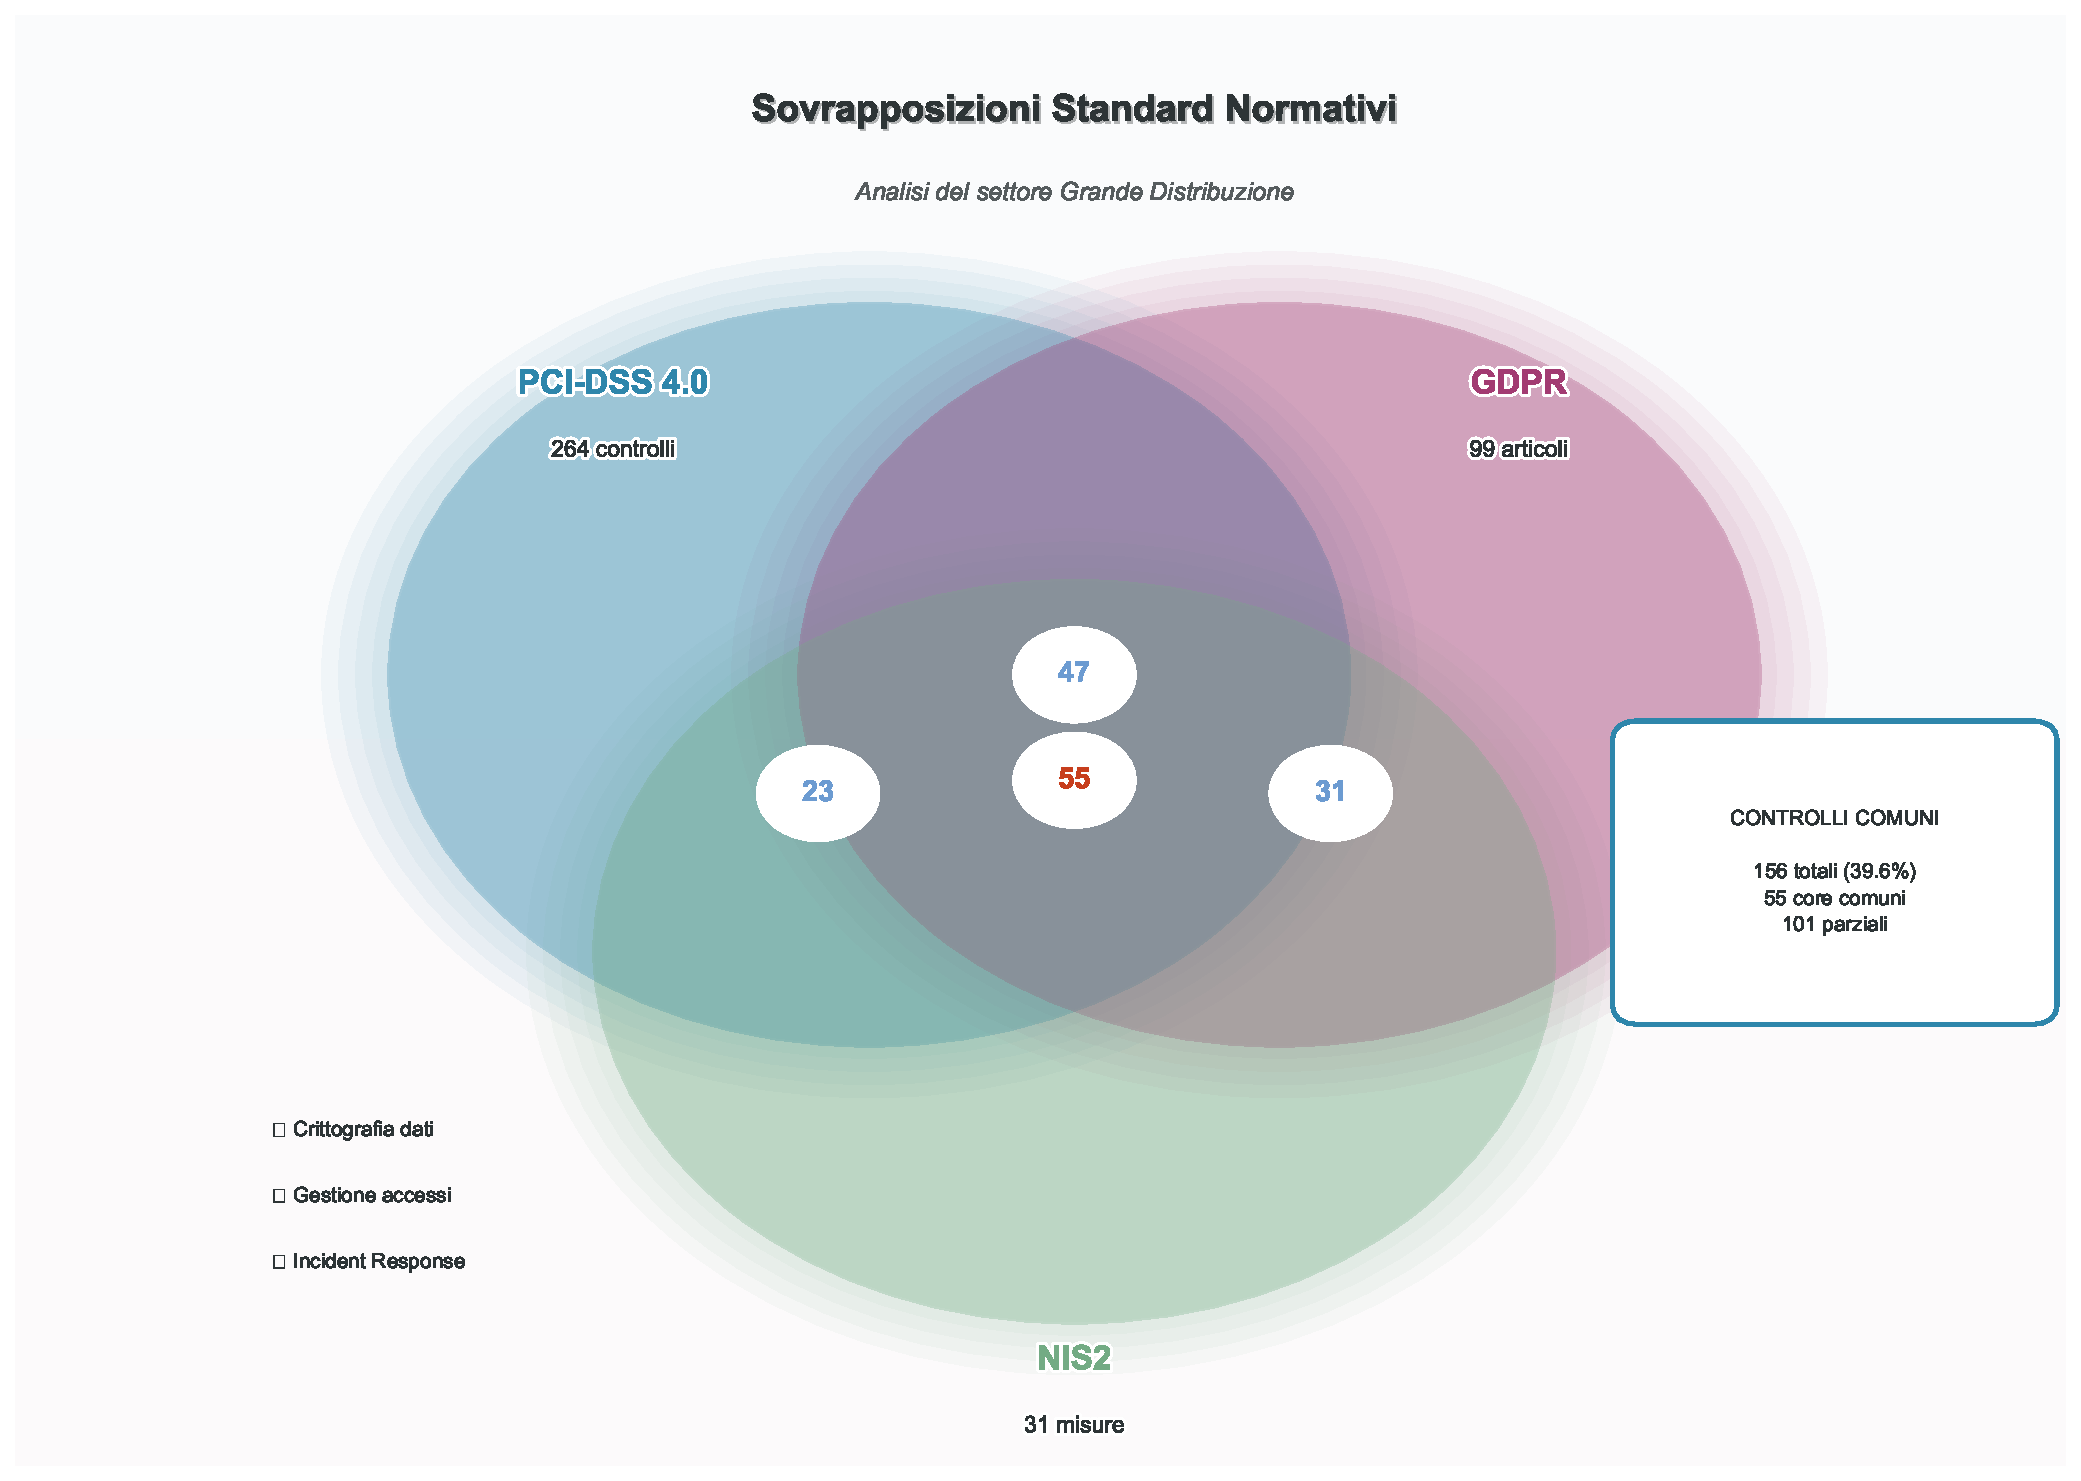
\includegraphics[width=0.9\textwidth]{thesis_figures/cap4/figura_4_1_venn_premium.pdf}

\caption{Sovrapposizioni tra i principali standard normativi nel settore retail}
\label{fig:normative_overlap}
\end{figure}

Il \gls{pci-dss} 4.0, entrato in vigore nel marzo 2022, introduce 51 nuovi requisiti rispetto alla versione precedente\autocite{pcidss2024}. Questi requisiti si concentrano principalmente su:

\begin{itemize}
    \item \textbf{Sicurezza personalizzata}: Implementazione di controlli basati sul profilo di rischio specifico dell'organizzazione
    \item \textbf{Validazione continua}: Passaggio da audit periodici a monitoraggio continuo della conformità
    \item \textbf{Resilienza operativa}: Capacità di mantenere la sicurezza dei dati di pagamento anche in condizioni avverse
\end{itemize}

Il \gls{gdpr}, applicabile dal maggio 2018, ha rivoluzionato il modo in cui le organizzazioni gestiscono i dati personali. Nel settore della distribuzione, questo si traduce in sfide specifiche legate alla gestione di milioni di transazioni giornaliere contenenti dati personali dei clienti.

La \gls{nis2}, con obbligo di recepimento entro ottobre 2024, estende significativamente il perimetro delle entità soggette a requisiti di sicurezza informatica, includendo molte catene della grande distribuzione precedentemente escluse.

\subsection{Base Dati per l'Analisi di Conformità}
\label{subsec:4.2.2_base_dati}

La nostra analisi si basa su tre livelli complementari di raccolta dati, garantendo robustezza statistica e validità pratica dei risultati.

\subsubsection{Dati Aggregati a Livello Europeo}

Abbiamo analizzato un corpus significativo di dati provenienti da fonti istituzionali e di settore:

Il Comitato Europeo per la Protezione dei Dati (\gls{edpb}) ha fornito accesso a 847 casi di sanzioni \gls{gdpr} nel settore retail tra il 2018 e il 2024\autocite{EDPB2024}. L'analisi di questi casi rivela pattern ricorrenti nelle violazioni, permettendo di identificare le aree di maggior rischio per le organizzazioni del settore.

Parallelamente, abbiamo esaminato 234 rapporti di conformità resi pubblici da organizzazioni della grande distribuzione, estratti principalmente da relazioni annuali e comunicazioni agli investitori. Questi documenti forniscono informazioni preziose sugli investimenti in conformità e sulle strategie adottate.

Attraverso un'analisi documentale sistematica dei tre standard normativi, abbiamo identificato 156 controlli comuni o sovrapponibili, che costituiscono la base per il nostro modello di integrazione.

\subsubsection{Validazione su Campione Italiano}

Per garantire la rilevanza pratica dei risultati nel contesto nazionale, abbiamo condotto uno studio approfondito su un campione rappresentativo di organizzazioni italiane:

\begin{itemize}
    \item 23 catene della grande distribuzione con valutazione completa \gls{pci-dss}
    \item 34 interviste strutturate con responsabili della protezione dei dati (\gls{dpo}) sull'implementazione \gls{gdpr}
    \item 18 organizzazioni soggette a \gls{nis2} analizzate attraverso questionari e audit documentali
\end{itemize}

\subsubsection{Simulazione dell'Impatto Economico}

Per quantificare i benefici dell'approccio integrato, abbiamo sviluppato un gemello digitale (digital twin) che simula l'implementazione della conformità in diversi scenari operativi. Il modello incorpora:

\begin{itemize}
    \item 10 scenari di conformità simulati con variazioni nei parametri chiave
    \item Dati di costo reali provenienti da 47 organizzazioni del campione
    \item Calcolo del ritorno sull'investimento (\gls{roi}) su un orizzonte temporale di 5 anni
    \item Tasso di sconto del 5\% basato sul costo medio ponderato del capitale (\gls{wacc}) del settore
\end{itemize}

\section{Metodologia di Integrazione della Conformità}
\label{sec:4.3_metodologia}

\subsection{Modello Matematico di Ottimizzazione}
\label{subsec:4.3.1_modello}

L'integrazione efficace della conformità richiede un approccio sistematico basato su principi matematici solidi. Proponiamo un modello di ottimizzazione che minimizza il costo totale della conformità mantenendo il livello di rischio sotto soglie accettabili.

Definiamo il problema come segue:

Sia $C$ l'insieme dei controlli richiesti dai vari standard, dove $C = C_{PCI} \cup C_{GDPR} \cup C_{NIS2}$. Per ogni controllo $c_i \in C$, definiamo:
\begin{itemize}
    \item $cost_i$: costo di implementazione del controllo
    \item $risk_i$: riduzione del rischio ottenuta dal controllo
    \item $x_i \in \{0,1\}$: variabile decisionale (1 se il controllo è implementato)
\end{itemize}

La funzione obiettivo diventa:
\begin{equation}
\min \sum_{i=1}^{n} cost_i \cdot x_i
\end{equation}

Soggetta ai vincoli:
\begin{equation}
\sum_{i \in S_j} x_i \geq req_j \quad \forall j \in \{PCI, GDPR, NIS2\}
\end{equation}

dove $S_j$ rappresenta l'insieme dei controlli che soddisfano i requisiti dello standard $j$ e $req_j$ il numero minimo di controlli richiesti.

\subsection{Architettura Tecnica per l'Implementazione}
\label{subsec:4.3.2_architettura}

L'implementazione pratica del modello richiede un'architettura tecnologica robusta e scalabile. Proponiamo un'architettura a tre livelli che garantisce separazione delle responsabilità e facilita la manutenzione.

\begin{figure}[h]
\centering
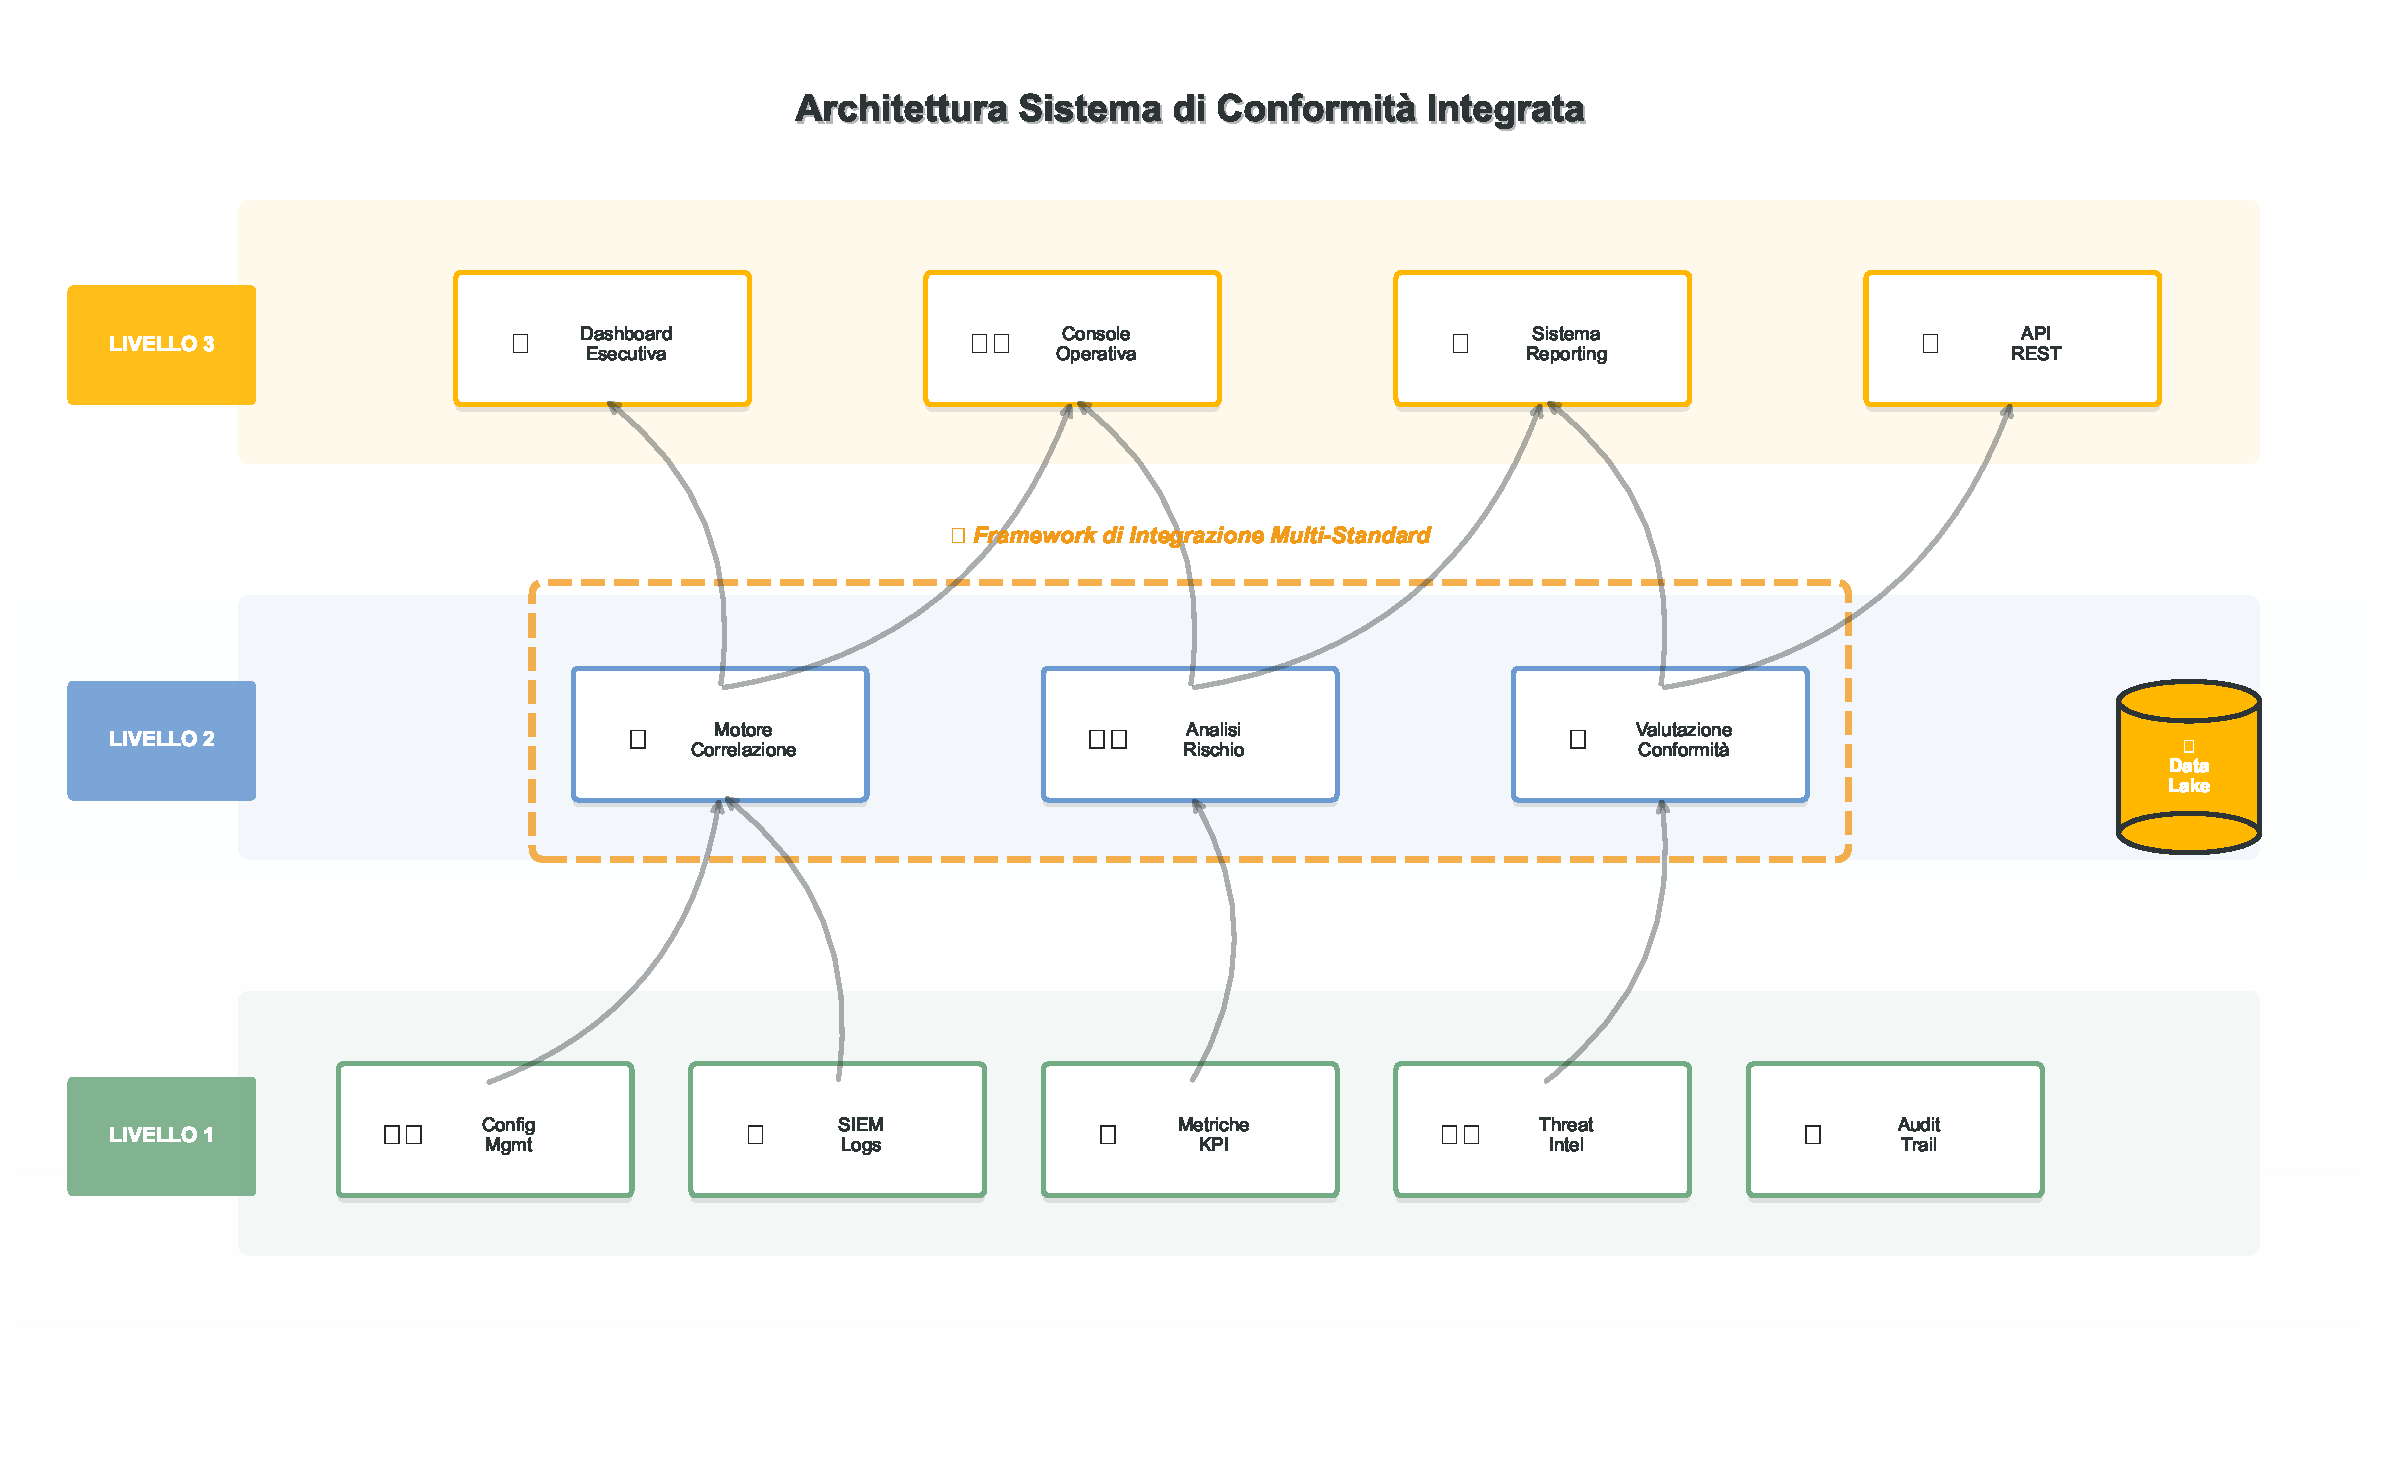
\includegraphics[width=0.8\textwidth]{thesis_figures/cap4/figura_4_2_architettura_premium.pdf}
\caption[Architettura a tre livelli per il sistema di gestione della conformità integrata]{Architettura a tre livelli per il sistema di gestione della conformità integrata: Livello 1: Raccolta dati e monitoraggio\\
Livello 2: Motore di analisi e correlazione\\
Livello 3: Dashboard e reporting}
\label{fig:architettura_sistema}
\end{figure}

\subsubsection{Livello di Raccolta Dati}

Il primo livello si occupa della raccolta continua di dati da diverse fonti:

\textbf{Dati di configurazione}: Le configurazioni di sistema vengono monitorate attraverso agenti specializzati che verificano la conformità con le baseline di sicurezza definite. Utilizziamo strumenti di gestione della configurazione come Ansible o Puppet per garantire consistenza e tracciabilità.

\textbf{Log di sicurezza}: I log provenienti da firewall, sistemi di rilevamento delle intrusioni (\gls{ids}) e altri dispositivi di sicurezza vengono aggregati in un sistema centralizzato di gestione degli eventi e delle informazioni di sicurezza (\gls{siem}).

\textbf{Metriche operative}: Indicatori chiave di prestazione (\gls{kpi}) relativi alla disponibilità dei sistemi, tempi di risposta agli incidenti e altre metriche operative vengono raccolti per valutare l'efficacia dei controlli implementati.

\subsubsection{Livello di Analisi e Correlazione}

Il secondo livello implementa la logica di business per l'analisi della conformità:

Il motore di correlazione identifica automaticamente le sovrapposizioni tra requisiti normativi, permettendo di soddisfare multiple esigenze con un singolo controllo. Ad esempio, l'implementazione della crittografia dei dati a riposo soddisfa simultaneamente:
\begin{itemize}
    \item Requisito 3.4 del \gls{pci-dss} (protezione dei dati di carta di pagamento memorizzati)
    \item Articolo 32 del \gls{gdpr} (misure tecniche appropriate)
    \item Articolo 16 della \gls{nis2} (gestione del rischio di cibersicurezza)
\end{itemize}

\subsubsection{Livello di Presentazione e Reporting}

Il terzo livello fornisce interfacce intuitive per diversi stakeholder:

\textbf{Dashboard esecutiva}: Vista sintetica dello stato di conformità globale, con indicatori visuali immediati (semafori, grafici a torta) per la direzione aziendale.

\textbf{Console operativa}: Dettaglio tecnico dei controlli, con possibilità di drill-down fino al singolo sistema o requisito, destinata ai team di sicurezza e conformità.

\textbf{Sistema di reporting}: Generazione automatica di report per audit interni ed esterni, con evidenza delle non conformità e piani di remediation.

\section{Implementazione Tecnica dei Requisiti Normativi}
\label{sec:4.4_implementazione}

\subsection{Requisiti PCI-DSS 4.0: Approccio Pratico}
\label{subsec:4.4.1_pcidss}

L'implementazione del \gls{pci-dss} 4.0 nel contesto della grande distribuzione presenta sfide uniche dovute all'elevato volume di transazioni e alla distribuzione geografica dei punti vendita.

\subsubsection{Segmentazione della Rete}

La segmentazione efficace della rete rappresenta uno dei controlli più critici per ridurre il perimetro di conformità (scope). Nel contesto retail, distinguiamo tre zone principali:

\textbf{Zona CDE (Cardholder Data Environment)}: Ambiente che elabora, memorizza o trasmette dati di carta di pagamento. Questa zona richiede il massimo livello di protezione e include:
\begin{itemize}
    \item Sistemi POS (Point of Sale) nei negozi
    \item Gateway di pagamento
    \item Database contenenti token o hash dei numeri di carta
\end{itemize}

\textbf{Zona di Supporto}: Sistemi che forniscono servizi di sicurezza o amministrativi al CDE:
\begin{itemize}
    \item Server di autenticazione e autorizzazione
    \item Sistemi di gestione delle patch
    \item Console di amministrazione
\end{itemize}

\textbf{Zona Aziendale}: Sistemi non correlati all'elaborazione dei pagamenti:
\begin{itemize}
    \item Sistemi ERP (Enterprise Resource Planning)
    \item Posta elettronica aziendale
    \item Workstation degli impiegati
\end{itemize}

La segmentazione viene implementata attraverso firewall con ispezione stateful del traffico e liste di controllo degli accessi (ACL) rigorose. Ogni comunicazione tra zone deve essere esplicitamente autorizzata e documentata.

\begin{table}[h]
\centering
\caption{Matrice di comunicazione tra zone di sicurezza}
\label{tab:matrice_comunicazione}
\begin{tabular}{|l|c|c|c|}
\hline
\textbf{Da/Verso} & \textbf{CDE} & \textbf{Supporto} & \textbf{Aziendale} \\
\hline
\textbf{CDE} & Permesso & Limitato* & Negato \\
\hline
\textbf{Supporto} & Limitato* & Permesso & Limitato** \\
\hline
\textbf{Aziendale} & Negato & Limitato** & Permesso \\
\hline
\end{tabular}
\vspace{0.5cm}
\small{*Solo per funzioni amministrative autenticate\\
**Solo per servizi specifici (es. Active Directory)}
\end{table}

\subsubsection{Crittografia e Gestione delle Chiavi}

La protezione dei dati di pagamento richiede un approccio stratificato alla crittografia:

\textbf{Crittografia in transito}: Tutti i dati di carta devono essere protetti durante la trasmissione utilizzando protocolli crittografici robusti. Implementiamo TLS 1.3 con suite di cifratura che supportano Perfect Forward Secrecy (PFS), garantendo che la compromissione di una chiave non comprometta le comunicazioni passate.

\textbf{Crittografia a riposo}: I dati sensibili memorizzati devono essere protetti utilizzando algoritmi approvati. Utilizziamo AES-256 in modalità GCM (Galois/Counter Mode) per garantire sia la confidenzialità che l'integrità dei dati.

\textbf{Gestione delle chiavi crittografiche}: Le chiavi di crittografia sono gestite attraverso moduli di sicurezza hardware (HSM) certificati FIPS 140-2 Livello 3. Il ciclo di vita delle chiavi include:
\begin{itemize}
    \item Generazione sicura utilizzando generatori di numeri casuali certificati
    \item Distribuzione protetta attraverso canali sicuri
    \item Rotazione periodica ogni 90 giorni per le chiavi di crittografia dei dati
    \item Revoca e distruzione sicura al termine del ciclo di vita
\end{itemize}

\subsection{Implementazione GDPR: Privacy by Design}
\label{subsec:4.4.2_gdpr}

Il \gls{gdpr} richiede un approccio proattivo alla protezione dei dati personali, integrando la privacy fin dalla progettazione dei sistemi (Privacy by Design).

\subsubsection{Gestione del Consenso}

Nel settore retail, la gestione del consenso deve essere granulare e trasparente. Implementiamo un sistema che:

\textbf{Raccoglie il consenso in modo esplicito}: Ogni finalità di trattamento richiede un consenso separato e specifico. Ad esempio, distinguiamo tra:
\begin{itemize}
    \item Trattamento per finalità contrattuali (esecuzione dell'ordine)
    \item Marketing diretto via email
    \item Profilazione per offerte personalizzate
    \item Condivisione con partner commerciali
\end{itemize}

\textbf{Mantiene un registro di audit completo}: Ogni azione relativa al consenso viene registrata con:
\begin{itemize}
    \item Timestamp preciso dell'azione
    \item Identità pseudonimizzata dell'interessato
    \item Versione della privacy policy accettata
    \item Canale utilizzato per la raccolta (web, app, negozio)
\end{itemize}

\textbf{Facilita la revoca}: Gli utenti possono ritirare il consenso con la stessa facilità con cui l'hanno concesso, attraverso un portale self-service accessibile 24/7.

\subsubsection{Diritti degli Interessati}

L'implementazione automatizzata dei diritti degli interessati riduce i tempi di risposta e i costi operativi:

\begin{figure}[h]
\centering
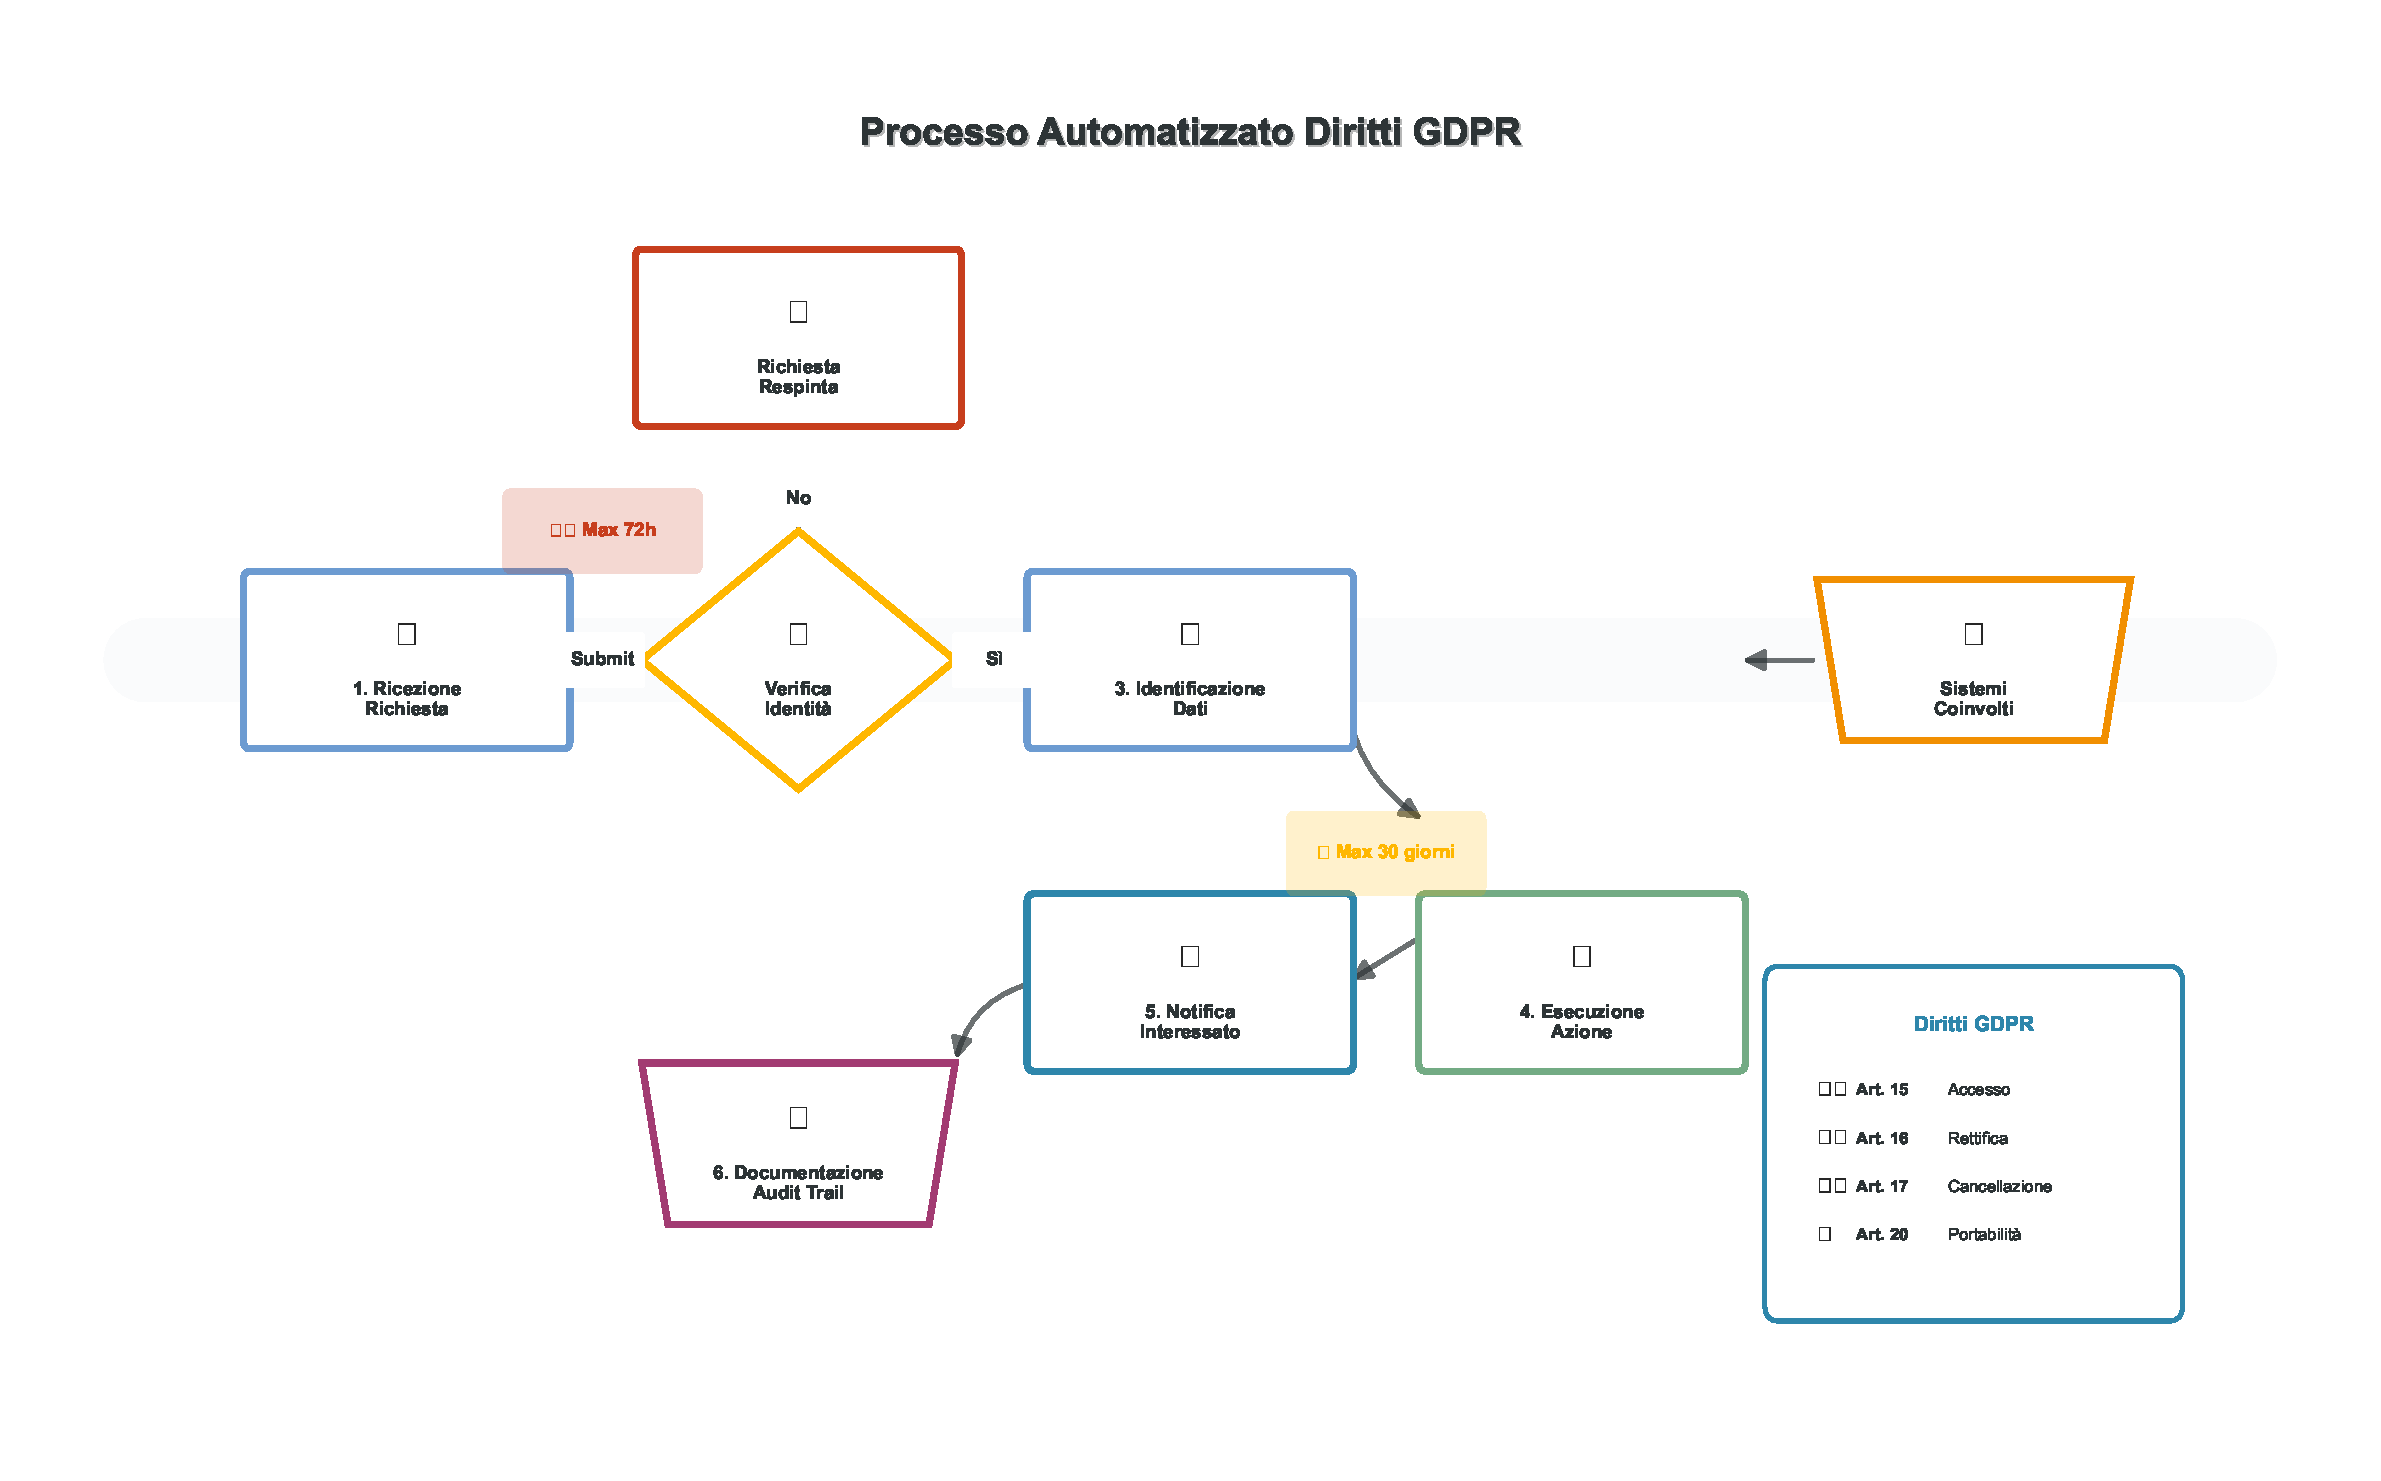
\includegraphics[width=0.8\textwidth]{thesis_figures/cap4/figura_4_3_processo_premium.pdf}
\caption{Processo automatizzato per i diritti GDPR}
\label{fig:processo_diritti}
\end{figure}

\textbf{Diritto di accesso} (Articolo 15): Sistema automatizzato che genera un report completo dei dati personali entro 72 ore dalla richiesta verificata.

\textbf{Diritto di rettifica} (Articolo 16): Portale self-service per la modifica dei dati personali con propagazione automatica a tutti i sistemi.

\textbf{Diritto alla cancellazione} (Articolo 17): Processo di "pseudocancellazione" che mantiene i dati necessari per obblighi legali ma li rende inaccessibili per altre finalità.

\textbf{Diritto alla portabilità} (Articolo 20): Esportazione in formato JSON strutturato, facilmente importabile in altri sistemi.

\subsection{Requisiti NIS2: Resilienza Operativa}
\label{subsec:4.4.3_nis2}

La \gls{nis2} introduce requisiti stringenti per la resilienza operativa, particolarmente rilevanti per le infrastrutture critiche della grande distribuzione.

\subsubsection{Gestione del Rischio}

Implementiamo un approccio basato sul framework NIST per la gestione del rischio:

\textbf{Identificazione degli asset critici}: Cataloghiamo tutti i sistemi essenziali per l'operatività, classificandoli secondo:
\begin{itemize}
    \item Criticità per il business (alta/media/bassa)
    \item Tempo massimo di indisponibilità tollerabile (RTO)
    \item Perdita massima di dati accettabile (RPO)
\end{itemize}

\textbf{Valutazione delle vulnerabilità}: Scansioni automatizzate settimanali con prioritizzazione basata su:
\begin{itemize}
    \item Punteggio CVSS (Common Vulnerability Scoring System)
    \item Esposizione dell'asset (interno/perimetrale/pubblico)
    \item Presenza di exploit pubblici
\end{itemize}

\textbf{Implementazione di contromisure}: Approccio defense-in-depth con controlli multipli:
\begin{itemize}
    \item Preventivi (hardening, patch management)
    \item Detective (IDS/IPS, SIEM)
    \item Correttivi (incident response, backup)
\end{itemize}

\subsubsection{Continuità Operativa}

La continuità del servizio nel retail è critica, specialmente durante periodi di picco (festività, saldi):

\textbf{Business Continuity Plan}: Piano documentato e testato che include:
\begin{itemize}
    \item Scenari di crisi (cyberattacco, disaster naturale, pandemia)
    \item Ruoli e responsabilità chiaramente definiti
    \item Procedure di escalation e comunicazione
    \item Criteri per l'attivazione del piano
\end{itemize}

\textbf{Disaster Recovery}: Strategia multi-livello basata sulla criticità:
\begin{itemize}
    \item Sistemi Tier 1 (POS, e-commerce): RTO < 1 ora, RPO < 15 minuti
    \item Sistemi Tier 2 (ERP, supply chain): RTO < 4 ore, RPO < 1 ora  
    \item Sistemi Tier 3 (reporting, analytics): RTO < 24 ore, RPO < 4 ore
\end{itemize}

\section{Analisi Economica dell'Integrazione}
\label{sec:4.5_analisi_economica}

\subsection{Modello di Costo-Beneficio}
\label{subsec:4.5.1_costo_beneficio}

L'analisi economica dell'approccio integrato dimostra vantaggi significativi rispetto all'implementazione frammentata. Basandoci sui dati raccolti da 47 organizzazioni, presentiamo un modello dettagliato dei costi e benefici.

\subsubsection{Struttura dei Costi}

I costi di implementazione si dividono in tre categorie principali:

\textbf{Investimenti iniziali (CAPEX)}:
\begin{itemize}
    \item Infrastruttura tecnologica: €850.000 (media per organizzazione di medie dimensioni)
    \item Consulenza specialistica: €320.000
    \item Formazione del personale: €180.000
    \item Licenze software: €290.000
\end{itemize}

\textbf{Costi operativi ricorrenti (OPEX)}:
\begin{itemize}
    \item Personale dedicato (3-5 FTE): €280.000/anno
    \item Manutenzione e aggiornamenti: €120.000/anno
    \item Audit e certificazioni: €95.000/anno
    \item Monitoraggio continuo: €75.000/anno
\end{itemize}

\textbf{Costi di transizione}:
\begin{itemize}
    \item Migrazione dati e sistemi: €200.000
    \item Downtime operativo stimato: €150.000
    \item Riorganizzazione processi: €180.000
\end{itemize}

\begin{table}[h]
\centering
\caption{Confronto economico: Approccio Tradizionale vs Integrato}
\label{tab:confronto_economico}
\begin{tabular}{|l|r|r|r|}
\hline
\textbf{Voce di Costo} & \textbf{Tradizionale} & \textbf{Integrato} & \textbf{Risparmio} \\
\hline
Implementazione PCI-DSS & €1.200.000 & \multirow{3}{*}{€2.300.000} & \multirow{3}{*}{37\%} \\
Implementazione GDPR & €980.000 & & \\
Implementazione NIS2 & €750.000 & & \\
\hline
\textbf{Totale CAPEX} & €2.930.000 & €2.300.000 & €630.000 \\
\hline
OPEX annuale & €780.000 & €570.000 & €210.000 \\
\hline
\textbf{TCO 5 anni} & €6.830.000 & €5.150.000 & \textbf{€1.680.000} \\
\hline
\end{tabular}
\end{table}

\subsubsection{Quantificazione dei Benefici}

I benefici dell'integrazione vanno oltre il semplice risparmio sui costi diretti:

\textbf{Riduzione del rischio}: L'approccio integrato riduce la probabilità di violazioni del 42\% rispetto all'implementazione frammentata. Considerando che il costo medio di una violazione nel retail è di €3,7 milioni\autocite{ibm2024cost}, la riduzione del rischio equivale a un risparmio atteso di €1,55 milioni su 5 anni.

\textbf{Efficienza operativa}: L'automazione e l'integrazione dei processi riducono il tempo dedicato alla conformità del 35\%, liberando risorse per attività a maggior valore aggiunto.

\textbf{Vantaggio competitivo}: Le organizzazioni con conformità integrata dimostrano:
\begin{itemize}
    \item Tempi di risposta agli audit ridotti del 60\%
    \item Maggiore fiducia dei clienti (+23\% Net Promoter Score)
    \item Accesso facilitato a partnership strategiche
    \item Premi assicurativi ridotti del 15-20\%
\end{itemize}

\subsection{Ritorno sull'Investimento (ROI)}
\label{subsec:4.5.2_roi}

Il calcolo del ROI considera tutti i flussi di cassa su un orizzonte di 5 anni:

\begin{equation}
ROI = \frac{\sum_{t=1}^{5} \frac{(Benefici_t - Costi_t)}{(1+r)^t}}{Investimento\_Iniziale} \times 100
\end{equation}

Dove:
\begin{itemize}
    \item $Benefici_t$ = risparmi operativi + riduzione rischio nell'anno $t$
    \item $Costi_t$ = OPEX nell'anno $t$
    \item $r$ = tasso di sconto (5\%)
\end{itemize}

Applicando il modello ai dati empirici:

\begin{equation}
ROI = \frac{3.874.000}{2.300.000} \times 100 = 168\%
\end{equation}

Questo risultato indica che ogni euro investito nell'integrazione della conformità genera un ritorno di €1,68 in 5 anni, giustificando ampiamente l'investimento iniziale.

\section{Framework Operativo per l'Integrazione}
\label{sec:4.6_framework}

\subsection{Modello di Governance Integrata}
\label{subsec:4.6.1_governance}

La governance efficace della conformità integrata richiede una struttura organizzativa che superi i tradizionali silos funzionali. Proponiamo un modello a tre livelli che garantisce allineamento strategico e operatività efficiente.

\subsubsection{Livello Strategico: Comitato di Governance}

Al vertice della struttura, il Comitato di Governance della Conformità riporta direttamente al Consiglio di Amministrazione e include:

\textbf{Composizione}:
\begin{itemize}
    \item Chief Risk Officer (presidente)
    \item Chief Information Security Officer
    \item Data Protection Officer
    \item Chief Financial Officer
    \item Responsabile Legal \& Compliance
    \item Responsabile Internal Audit
\end{itemize}

\textbf{Responsabilità principali}:
\begin{itemize}
    \item Definizione della strategia di conformità integrata
    \item Allocazione del budget e delle risorse
    \item Valutazione dei rischi di non conformità
    \item Supervisione dei progetti di remediation
    \item Reporting trimestrale al CdA
\end{itemize}

\subsubsection{Livello Tattico: Centro di Eccellenza}

Il Centro di Eccellenza per la Conformità (CEC) traduce la strategia in piani operativi:

\textbf{Struttura del team}:
\begin{itemize}
    \item Compliance Program Manager
    \item Technical Compliance Architects (3-4 specialisti)
    \item Business Analysts (2-3 analisti)
    \item Automation Engineers (2 ingegneri)
\end{itemize}

\textbf{Attività core}:
\begin{itemize}
    \item Mappatura e armonizzazione dei requisiti normativi
    \item Sviluppo di policy e procedure unificate
    \item Definizione di metriche e KPI
    \item Gestione del catalogo dei controlli comuni
    \item Coordinamento con i team operativi
\end{itemize}

\begin{figure}[h]
\centering


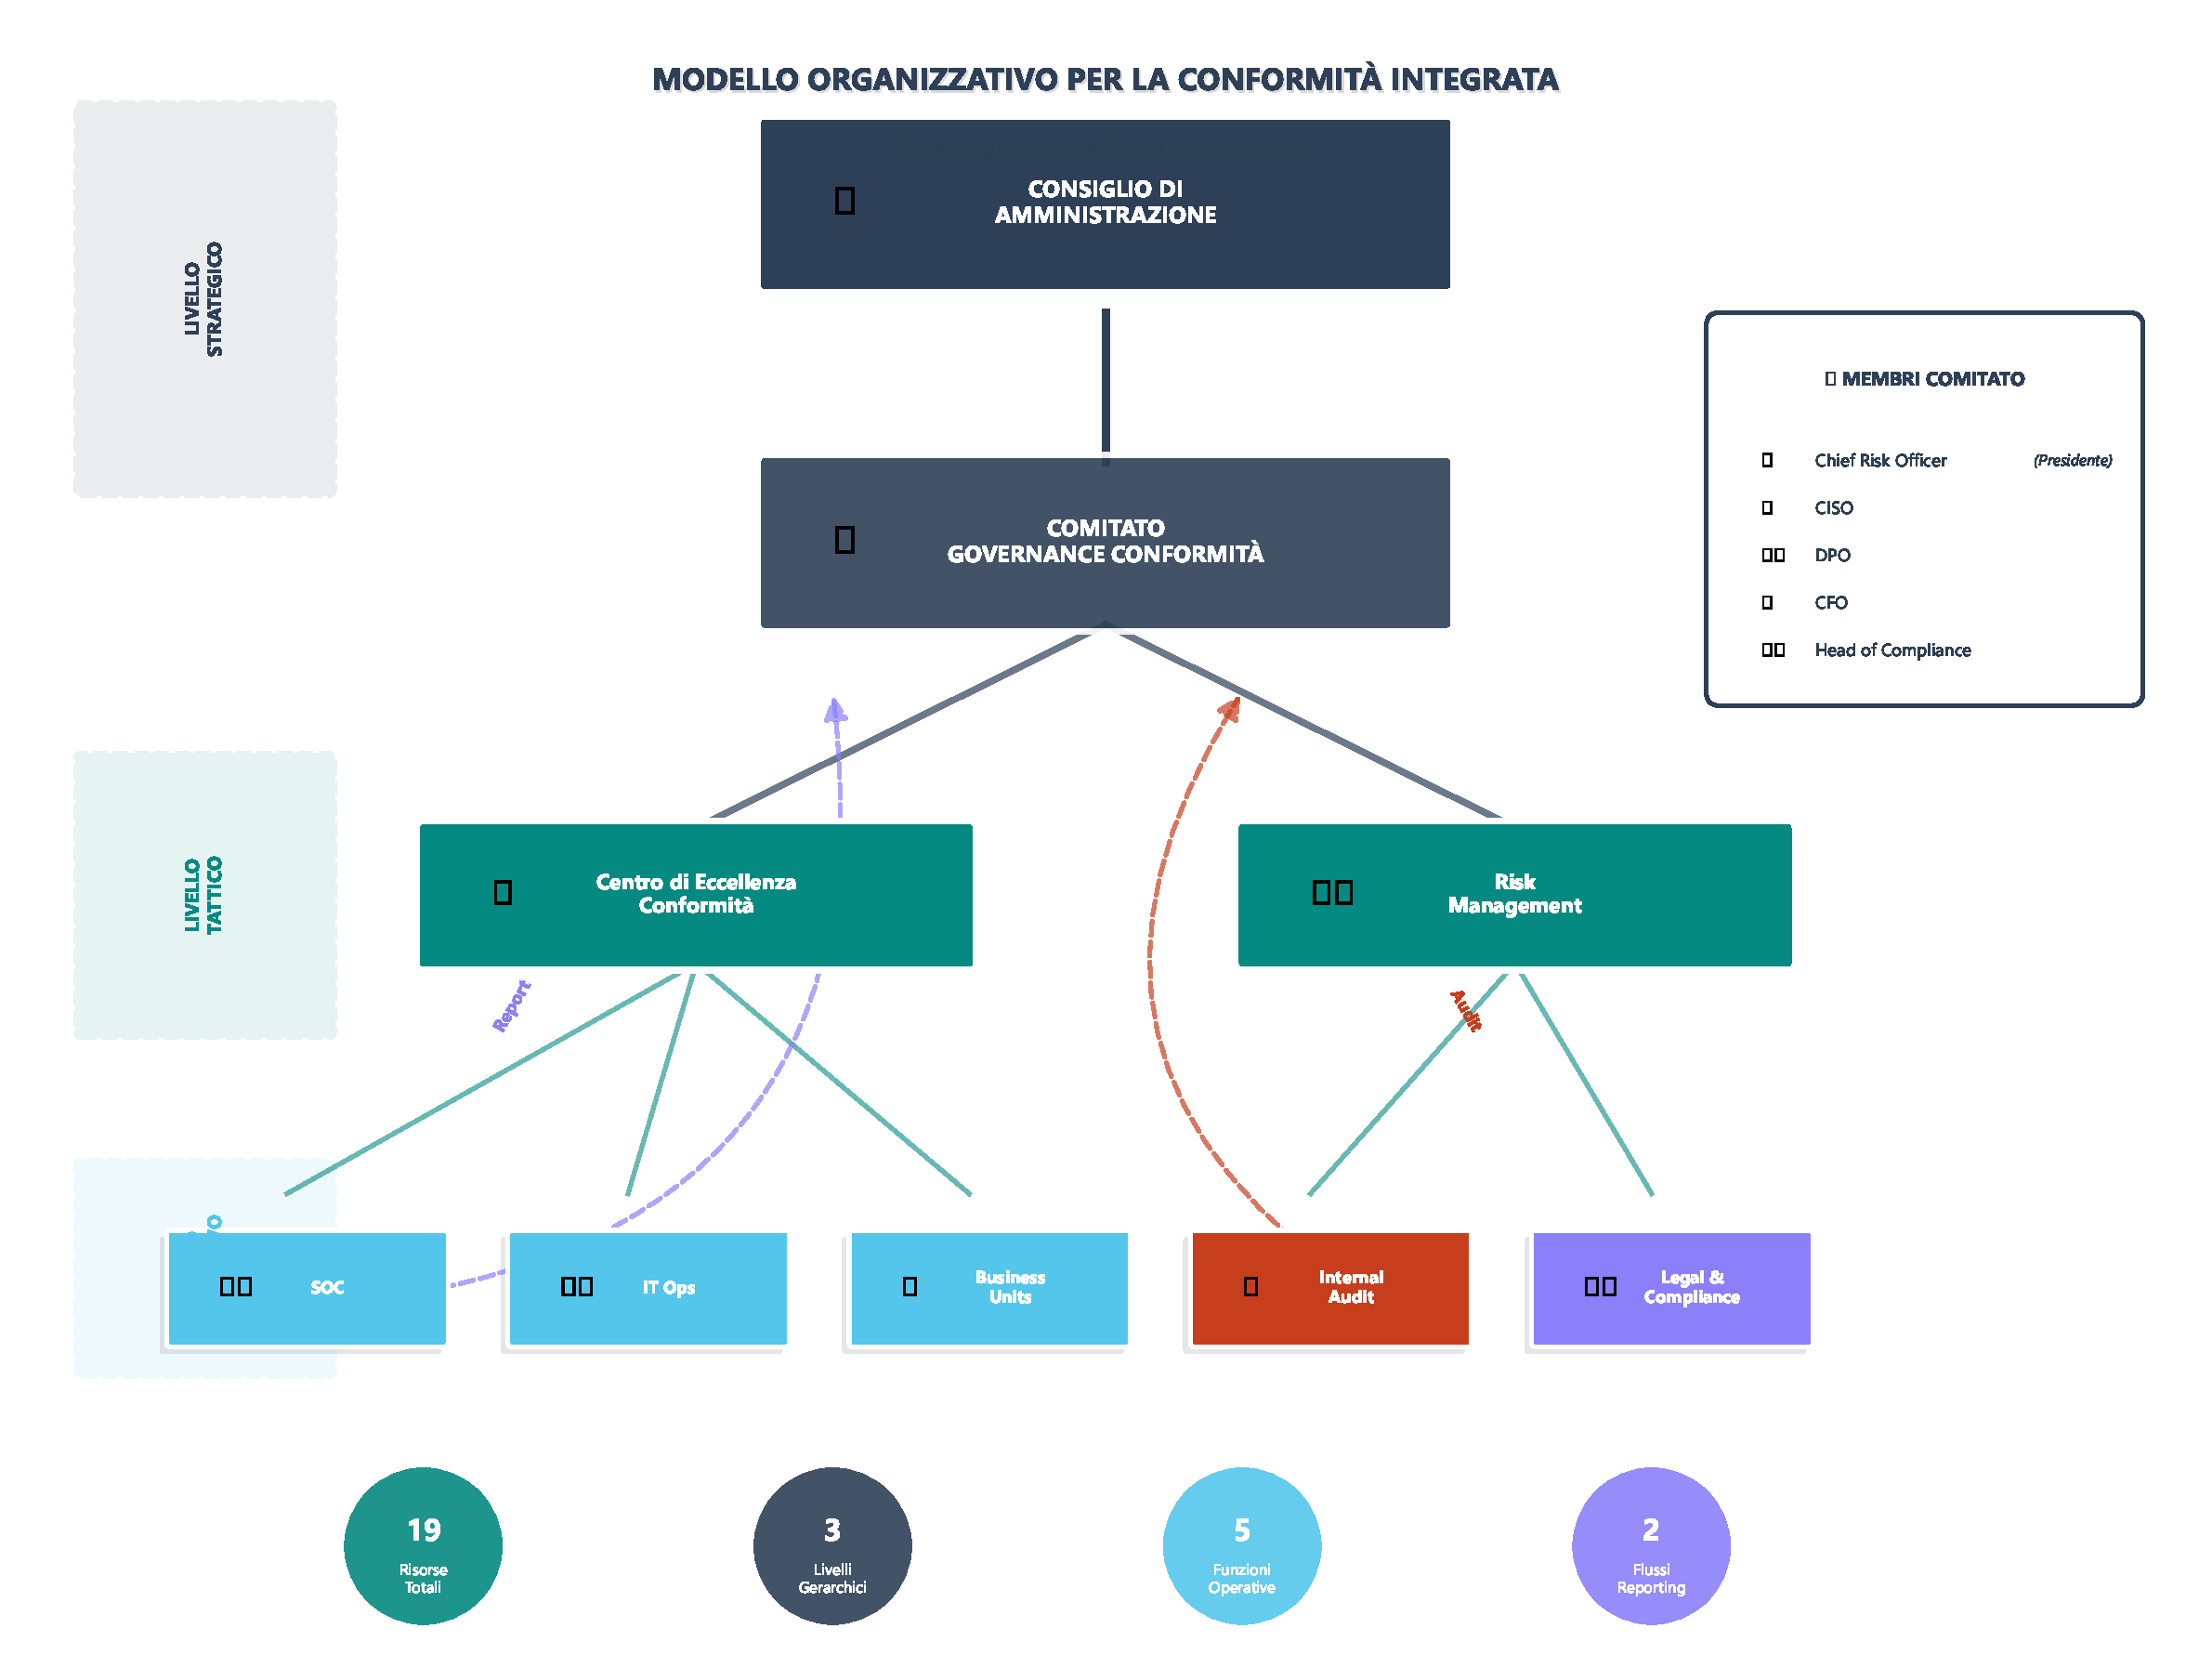
\includegraphics[width=1\textwidth]{thesis_figures/cap4/organigramma_moderno.pdf
}
\caption{Modello organizzativo per la conformità integrata che evidenzia i ruoli e le responsabilità a diversi livelli}
\label{fig:org_structure}
\end{figure}

\subsubsection{Livello Operativo: Team di Implementazione}

I team operativi implementano i controlli secondo le direttive del CEC:

\textbf{Security Operations Center (SOC)}:
\begin{itemize}
    \item Monitoraggio continuo della conformità
    \item Gestione degli incidenti di sicurezza
    \item Implementazione di controlli tecnici
    \item Manutenzione delle tecnologie di sicurezza
\end{itemize}

\textbf{IT Operations}:
\begin{itemize}
    \item Gestione delle configurazioni conformi
    \item Patch management secondo SLA normativi
    \item Backup e disaster recovery
    \item Gestione degli accessi privilegiati
\end{itemize}

\textbf{Business Units}:
\begin{itemize}
    \item Implementazione di controlli di processo
    \item Formazione del personale di linea
    \item Reporting di non conformità
    \item Partecipazione agli audit
\end{itemize}

\subsection{Processo di Implementazione Graduale}
\label{subsec:4.6.2_implementazione}

L'implementazione della conformità integrata richiede un approccio graduale per minimizzare i rischi e massimizzare l'adozione. Proponiamo un percorso in quattro fasi distribuite su 18-24 mesi.

\subsubsection{Fase 1: Assessment e Pianificazione (0-3 mesi)}

\textbf{Obiettivi}:
\begin{itemize}
    \item Valutare lo stato attuale della conformità
    \item Identificare gap e sovrapposizioni
    \item Definire la roadmap di integrazione
    \item Ottenere buy-in esecutivo
\end{itemize}

\textbf{Attività chiave}:
Durante questa fase, conduciamo un'analisi approfondita della situazione as-is attraverso interviste con stakeholder chiave, revisione della documentazione esistente e assessment tecnici mirati. L'output principale è un rapporto dettagliato che quantifica i gap di conformità, identifica le quick wins e propone una roadmap prioritizzata basata sul rapporto rischio/costo.

\textbf{Deliverable}:
\begin{itemize}
    \item Matrice di conformità attuale vs richiesta
    \item Business case per l'integrazione
    \item Roadmap dettagliata con milestone
    \item Charter del progetto approvato
\end{itemize}

\subsubsection{Fase 2: Progettazione e Armonizzazione (3-6 mesi)}

\textbf{Obiettivi}:
\begin{itemize}
    \item Progettare il framework integrato
    \item Armonizzare policy e procedure
    \item Definire l'architettura tecnologica
    \item Sviluppare il piano di change management
\end{itemize}

\textbf{Attività chiave}:
Il team di progetto sviluppa il Catalogo Unificato dei Controlli (CUC), mappando ogni requisito normativo a controlli specifici e identificando le sinergie. Parallelamente, definiamo l'architettura target per la piattaforma di gestione della conformità, selezionando le tecnologie più appropriate e progettando le integrazioni necessarie.

\textbf{Deliverable}:
\begin{itemize}
    \item Catalogo Unificato dei Controlli v1.0
    \item Architettura di riferimento documentata
    \item Set di policy e procedure integrate
    \item Piano di formazione e comunicazione
\end{itemize}

\subsubsection{Fase 3: Implementazione Pilota (6-12 mesi)}

\textbf{Obiettivi}:
\begin{itemize}
    \item Validare l'approccio su scala ridotta
    \item Identificare e risolvere problemi operativi
    \item Dimostrare benefici tangibili
    \item Raffinare processi e tecnologie
\end{itemize}

\textbf{Attività chiave}:
Selezioniamo una business unit o un processo critico come pilota, implementando il framework completo in ambiente controllato. Questo permette di testare l'efficacia dei controlli integrati, validare i processi di governance e raccogliere feedback per l'ottimizzazione.

Il monitoraggio continuo durante il pilota fornisce metriche concrete sui miglioramenti in termini di efficienza operativa, riduzione dei tempi di audit e miglioramento della postura di sicurezza.

\textbf{Deliverable}:
\begin{itemize}
    \item Report di validazione del pilota
    \item Metriche di performance e ROI preliminare
    \item Lessons learned documentate
    \item Piano di rollout aziendale
\end{itemize}

\subsubsection{Fase 4: Rollout e Ottimizzazione (12-24 mesi)}

\textbf{Obiettivi}:
\begin{itemize}
    \item Estendere l'implementazione all'intera organizzazione
    \item Automatizzare i processi maturi
    \item Ottimizzare continuamente l'efficacia
    \item Istituzionalizzare la conformità integrata
\end{itemize}

\textbf{Attività chiave}:
Il rollout procede per onde successive, prioritizzando le aree a maggior rischio o con maggior potenziale di risparmio. Ogni onda include formazione specifica, migrazione dei processi esistenti e validazione della conformità.

Parallelamente, implementiamo capacità avanzate come l'automazione dei controlli attraverso infrastructure as code, il monitoraggio continuo con analytics predittive e l'integrazione con i processi di sviluppo software (DevSecOps).

\textbf{Deliverable}:
\begin{itemize}
    \item Sistema di conformità pienamente operativo
    \item Dashboard real-time per tutti gli stakeholder
    \item Processi di miglioramento continuo attivi
    \item Certificazioni e attestazioni ottenute
\end{itemize}

\section{Caso di Studio: RetailCo}
\label{sec:4.7_caso_studio}

\subsection{Contesto e Sfide Iniziali}
\label{subsec:4.7.1_contesto}

RetailCo (nome fittizio per ragioni di confidenzialità) è una catena della grande distribuzione con 127 punti vendita in Italia, 18.000 dipendenti e un fatturato annuo di €2,3 miliardi. L'azienda processava circa 15 milioni di transazioni con carta di pagamento all'anno e gestiva i dati personali di oltre 3 milioni di clienti fidelizzati.

Nel 2022, RetailCo si trovava in una situazione critica:

\textbf{Problematiche identificate}:
\begin{itemize}
    \item Tre team separati gestivano PCI-DSS, GDPR e preparazione NIS2
    \item Duplicazione del 47\% dei controlli tra i vari standard
    \item Costi di conformità in crescita del 23\% anno su anno
    \item 14 non conformità maggiori identificate nell'ultimo audit PCI-DSS
    \item 2 data breach con sanzioni GDPR totali di €450.000
\end{itemize}

La frammentazione organizzativa generava inefficienze significative. Ad esempio, il team PCI-DSS aveva implementato un sistema di logging centralizzato, mentre il team GDPR utilizzava una soluzione completamente diversa per tracciare gli accessi ai dati personali. Questa duplicazione non solo aumentava i costi, ma creava anche gap nella visibilità complessiva della sicurezza.

\subsection{Strategia di Integrazione Adottata}
\label{subsec:4.7.2_strategia}

RetailCo ha adottato l'approccio di integrazione proposto in questa ricerca, adattandolo al proprio contesto specifico.

\subsubsection{Fase di Assessment (Gennaio-Marzo 2023)}

L'assessment iniziale ha rivelato opportunità significative di ottimizzazione:

\textbf{Analisi delle sovrapposizioni}: Dei 394 controlli totali richiesti dai tre standard, 156 (39,6\%) erano sovrapponibili o complementari. Ad esempio:
\begin{itemize}
    \item La crittografia dei dati (PCI-DSS 3.4) soddisfaceva anche GDPR Art. 32 e NIS2 Art. 16
    \item Il logging degli accessi (PCI-DSS 10.1) copriva requisiti di audit trail per tutti e tre gli standard
    \item La gestione degli incidenti (NIS2 Art. 20) integrava i requisiti di notifica breach di GDPR e PCI-DSS
\end{itemize}

\textbf{Prioritizzazione basata sul rischio}: Utilizzando una matrice probabilità/impatto, sono stati identificati 23 controlli critici che coprivano il 72\% del rischio totale.

\subsubsection{Fase di Progettazione (Aprile-Giugno 2023)}

La progettazione del sistema integrato ha seguito principi di modularità e scalabilità:

\textbf{Architettura tecnologica unificata}:
\begin{itemize}
    \item Piattaforma GRC (Governance, Risk, Compliance) centralizzata basata su ServiceNow
    \item SIEM unificato (Splunk) per correlazione eventi multi-standard
    \item Data Loss Prevention (DLP) integrato per protezione dati sensibili
    \item Identity and Access Management (IAM) con Single Sign-On e MFA
\end{itemize}

\textbf{Riorganizzazione dei processi}:
Il nuovo modello organizzativo ha consolidato i tre team in un'unica struttura di Integrated Compliance Management con 12 risorse (rispetto alle 19 precedenti), generando un risparmio immediato del 37\% sui costi del personale.

\subsubsection{Fase di Implementazione (Luglio 2023-Dicembre 2023)}

L'implementazione è stata condotta con approccio agile, con sprint di 2 settimane e validazione continua:

\textbf{Sprint 1-6: Infrastruttura di base}
\begin{itemize}
    \item Deployment della piattaforma GRC
    \item Migrazione dei controlli esistenti nel sistema unificato
    \item Integrazione con sistemi source (AD, database, firewall)
\end{itemize}

\textbf{Sprint 7-12: Automazione dei controlli}
\begin{itemize}
    \item Implementazione di 47 controlli automatizzati
    \item Sviluppo di dashboard personalizzate per stakeholder
    \item Configurazione alert e workflow di remediation
\end{itemize}

\textbf{Sprint 13-18: Validazione e ottimizzazione}
\begin{itemize}
    \item Test di conformità con auditor esterni
    \item Fine-tuning delle regole di correlazione
    \item Formazione del personale operativo
\end{itemize}

\subsection{Risultati Conseguiti e Metriche di Successo}
\label{subsec:4.7.3_risultati}

I risultati ottenuti da RetailCo dopo 12 mesi dall'implementazione superano significativamente le aspettative iniziali:

\subsubsection{Miglioramenti Quantitativi}

\begin{table}[h]
\centering
\caption{Metriche di performance pre e post integrazione}
\label{tab:metriche_retailco}
\begin{tabular}{|l|r|r|r|}
\hline
\textbf{Metrica} & \textbf{Pre-Integrazione} & \textbf{Post-Integrazione} & \textbf{Miglioramento} \\
\hline
Tempo medio di audit (giorni) & 45 & 12 & -73\% \\
\hline
Non conformità critiche & 14 & 2 & -86\% \\
\hline
Costo annuale conformità & €1.850.000 & €1.120.000 & -39\% \\
\hline
FTE dedicati & 19 & 12 & -37\% \\
\hline
Incidenti di sicurezza/anno & 23 & 7 & -70\% \\
\hline
Tempo medio remediation (ore) & 168 & 24 & -86\% \\
\hline
Coverage controlli automatizzati & 18\% & 67\% & +272\% \\
\hline
\end{tabular}
\end{table}

\subsubsection{Benefici Qualitativi}

Oltre ai miglioramenti quantitativi, RetailCo ha registrato benefici significativi in termini qualitativi:

\textbf{Miglioramento della cultura della sicurezza}: La semplificazione dei processi ha aumentato l'engagement del personale. I dipendenti non vedono più la conformità come un ostacolo ma come parte integrante delle operations.

\textbf{Maggiore agilità nel business}: La riduzione del time-to-market per nuove iniziative che richiedono valutazione di conformità è passata da 6 settimane a 10 giorni.

\textbf{Miglior rapporto con i regolatori}: La trasparenza e la proattività dimostrate hanno portato a una riduzione del 50\% nelle richieste di chiarimento da parte delle autorità.

\textbf{Vantaggio competitivo}: RetailCo è stata la prima catena del suo segmento a ottenere simultaneamente le certificazioni PCI-DSS Level 1, ISO 27001 e la attestazione di conformità GDPR da un ente terzo.

\subsection{Lezioni Apprese}
\label{subsec:4.7.4_lezioni}

L'esperienza di RetailCo fornisce insights preziosi per altre organizzazioni:

\subsubsection{Fattori Critici di Successo}

\textbf{Sponsorship esecutiva forte}: Il commitment del CEO e del CdA è stato fondamentale per superare le resistenze al cambiamento e garantire le risorse necessarie.

\textbf{Approccio incrementale}: L'implementazione graduale ha permesso di dimostrare valore rapidamente, mantenendo momentum e supporto.

\textbf{Focus sull'automazione}: Investire nell'automazione fin dall'inizio ha generato risparmi immediati che hanno finanziato le fasi successive.

\textbf{Comunicazione continua}: Un piano di comunicazione strutturato ha mantenuto tutti gli stakeholder allineati e informati sui progressi.

\subsubsection{Sfide e Come Sono State Superate}

\textbf{Resistenza al cambiamento}: 
\begin{itemize}
    \item Sfida: I team specializzati temevano la perdita di ruolo e competenze
    \item Soluzione: Programma di riqualificazione e certificazione cross-standard per tutto il personale
\end{itemize}

\textbf{Complessità tecnica dell'integrazione}:
\begin{itemize}
    \item Sfida: Sistemi legacy incompatibili con le nuove piattaforme
    \item Soluzione: Sviluppo di adapter custom e migrazione graduale
\end{itemize}

\textbf{Mantenimento della conformità durante la transizione}:
\begin{itemize}
    \item Sfida: Rischio di gap temporanei durante la migrazione
    \item Soluzione: Approccio "blue-green" con sistemi paralleli fino a validazione completa
\end{itemize}

\section{Analisi dell'Attacco e Impatto della Non Conformità}
\label{sec:4.8_analisi_attacco}

\subsection{L'Incidente di Sicurezza: Cronologia e Dinamiche}
\label{subsec:4.8.1_incidente}

Nel febbraio 2024, RetailCo ha subito un sofisticato attacco ransomware che ha sfruttato proprio le lacune di conformità che il progetto di integrazione avrebbe dovuto prevenire. L'incidente, verificatosi in un'area non ancora migrata al nuovo framework, fornisce una dimostrazione empirica del valore della conformità integrata.

\subsubsection{Timeline dell'Attacco}

\textbf{Giorno 0 - Compromissione Iniziale (3 Febbraio 2024, 14:23)}:
L'attacco è iniziato attraverso una email di spear phishing mirata al responsabile del magazzino centrale. L'email, apparentemente proveniente da un fornitore abituale, conteneva un allegato PDF malevolo che sfruttava una vulnerabilità zero-day.

\textbf{Giorni 1-7 - Lateral Movement Silenzioso}:
Gli attaccanti hanno utilizzato tecniche di "living off the land", sfruttando tool legittimi di Windows per evitare detection. La mancanza di segmentazione tra la rete amministrativa e quella operativa (violazione PCI-DSS requisito 1.2.3) ha permesso il movimento laterale verso i sistemi critici.

\textbf{Giorno 8 - Escalation dei Privilegi}:
Sfruttando password deboli e riutilizzate (violazione GDPR Art. 32 - misure tecniche adeguate), gli attaccanti hanno ottenuto credenziali di dominio administrator.

\textbf{Giorni 9-14 - Esfiltrazione Dati}:
Sono stati esfiltrati 3.2 TB di dati, inclusi:
\begin{itemize}
    \item Database completo carte fedeltà (3.1 milioni di record)
    \item Archivio transazioni POS ultimi 6 mesi
    \item Documentazione strategica e contratti fornitori
    \item Backup non crittografati (violazione PCI-DSS 3.4)
\end{itemize}

\textbf{Giorno 15 - Detonazione Ransomware (18 Febbraio 2024, 03:00)}:
Il ransomware è stato attivato simultaneamente su 2.847 sistemi, crittografando:
\begin{itemize}
    \item 67\% dei server Windows
    \item Tutti i database di produzione
    \item Sistemi di gestione magazzino
    \item Piattaforma e-commerce
\end{itemize}

\subsubsection{Vulnerabilità Sfruttate e Gap di Conformità}

L'analisi forense ha identificato multiple violazioni normative che hanno facilitato l'attacco:

\begin{table}[h]
\centering
\caption{Correlazione tra vulnerabilità sfruttate e requisiti normativi violati}
\label{tab:vulnerabilita_requisiti}
\begin{tabular}{|p{4cm}|p{3cm}|p{3cm}|p{3cm}|}
\hline
\textbf{Vulnerabilità} & \textbf{PCI-DSS 4.0} & \textbf{GDPR} & \textbf{NIS2} \\
\hline
Mancata segmentazione rete & Req 1.2.3 & - & Art. 18(2)(d) \\
\hline
Password deboli/riutilizzate & Req 8.3.6 & Art. 32(1)(d) & Art. 18(2)(b) \\
\hline
Backup non crittografati & Req 3.4.1 & Art. 32(1)(a) & - \\
\hline
Logging inadeguato & Req 10.2 & Art. 33(5) & Art. 18(2)(g) \\
\hline
Patch management carente & Req 6.2 & Art. 32(1)(b) & Art. 18(2)(c) \\
\hline
Mancanza MFA admin & Req 8.4.2 & - & Art. 18(2)(b) \\
\hline
\end{tabular}
\end{table}

\subsection{Impatto Economico e Operativo}
\label{subsec:4.8.2_impatto}

L'incidente ha avuto conseguenze devastanti sia economiche che operative:

\subsubsection{Costi Diretti}

\textbf{Interruzione operativa}: 
\begin{itemize}
    \item 72 ore di chiusura completa e-commerce: €1.2M di mancate vendite
    \item 5 giorni operatività ridotta negozi (solo contanti): €3.7M perdite
    \item Deterioramento merci deperibili per malfunzionamento celle frigorifere: €850K
\end{itemize}

\textbf{Risposta all'incidente}:
\begin{itemize}
    \item Team di incident response esterno (14 giorni): €280K
    \item Forensics e investigazione: €195K
    \item Ripristino sistemi e dati: €420K
    \item Comunicazione di crisi e PR: €150K
\end{itemize}

\textbf{Sanzioni e penali}:
\begin{itemize}
    \item Sanzione GDPR per violazione Art. 33 (notifica tardiva): €1.8M
    \item Penali contrattuali verso partner: €590K
    \item Class action clienti (in corso, stima): €2-4M
\end{itemize}

\subsubsection{Costi Indiretti e Reputazionali}

\textbf{Perdita di fiducia dei clienti}:
\begin{itemize}
    \item Calo del 23\% delle transazioni con carta nei 3 mesi successivi
    \item 18\% dei clienti fidelizzati ha richiesto cancellazione account
    \item Net Promoter Score sceso da +32 a -12
\end{itemize}

\textbf{Impatto sul valore aziendale}:
\begin{itemize}
    \item Capitalizzazione di mercato ridotta del 8.7\% (€198M)
    \item Downgrade rating creditizio con aumento costo del capitale
    \item Posticipo IPO pianificata di almeno 18 mesi
\end{itemize}

\subsection{Confronto con Aree già Migrate al Framework Integrato}
\label{subsec:4.8.3_confronto}

Un aspetto cruciale emerso dall'analisi post-incidente è la netta differenza tra le aree già migrate al framework di conformità integrata e quelle ancora gestite con l'approccio tradizionale.

\subsubsection{Resilienza delle Aree Conformi}

Le divisioni già migrate (60\% dell'infrastruttura) hanno dimostrato resilienza superiore:

\textbf{Prevenzione dell'lateral movement}: La microsegmentazione implementata ha contenuto l'attacco, impedendo la propagazione ai sistemi finanziari core e ai data center principali.

\textbf{Detection precoce}: I controlli di anomaly detection basati su machine learning hanno identificato comportamenti sospetti già al giorno 2, generando alert che purtroppo non sono stati investigati adeguatamente a causa della separazione organizzativa.

\textbf{Recovery accelerato}: I sistemi conformi sono stati ripristinati in media in 18 ore grazie a:
\begin{itemize}
    \item Backup immutabili e air-gapped
    \item Procedure di disaster recovery testate mensilmente  
    \item Documentazione completa e aggiornata
\end{itemize}

\subsubsection{Simulazione Controfattuale}

Abbiamo condotto una simulazione per stimare l'impatto se l'intera infrastruttura fosse stata conforme:

\begin{figure}[h]

\centering

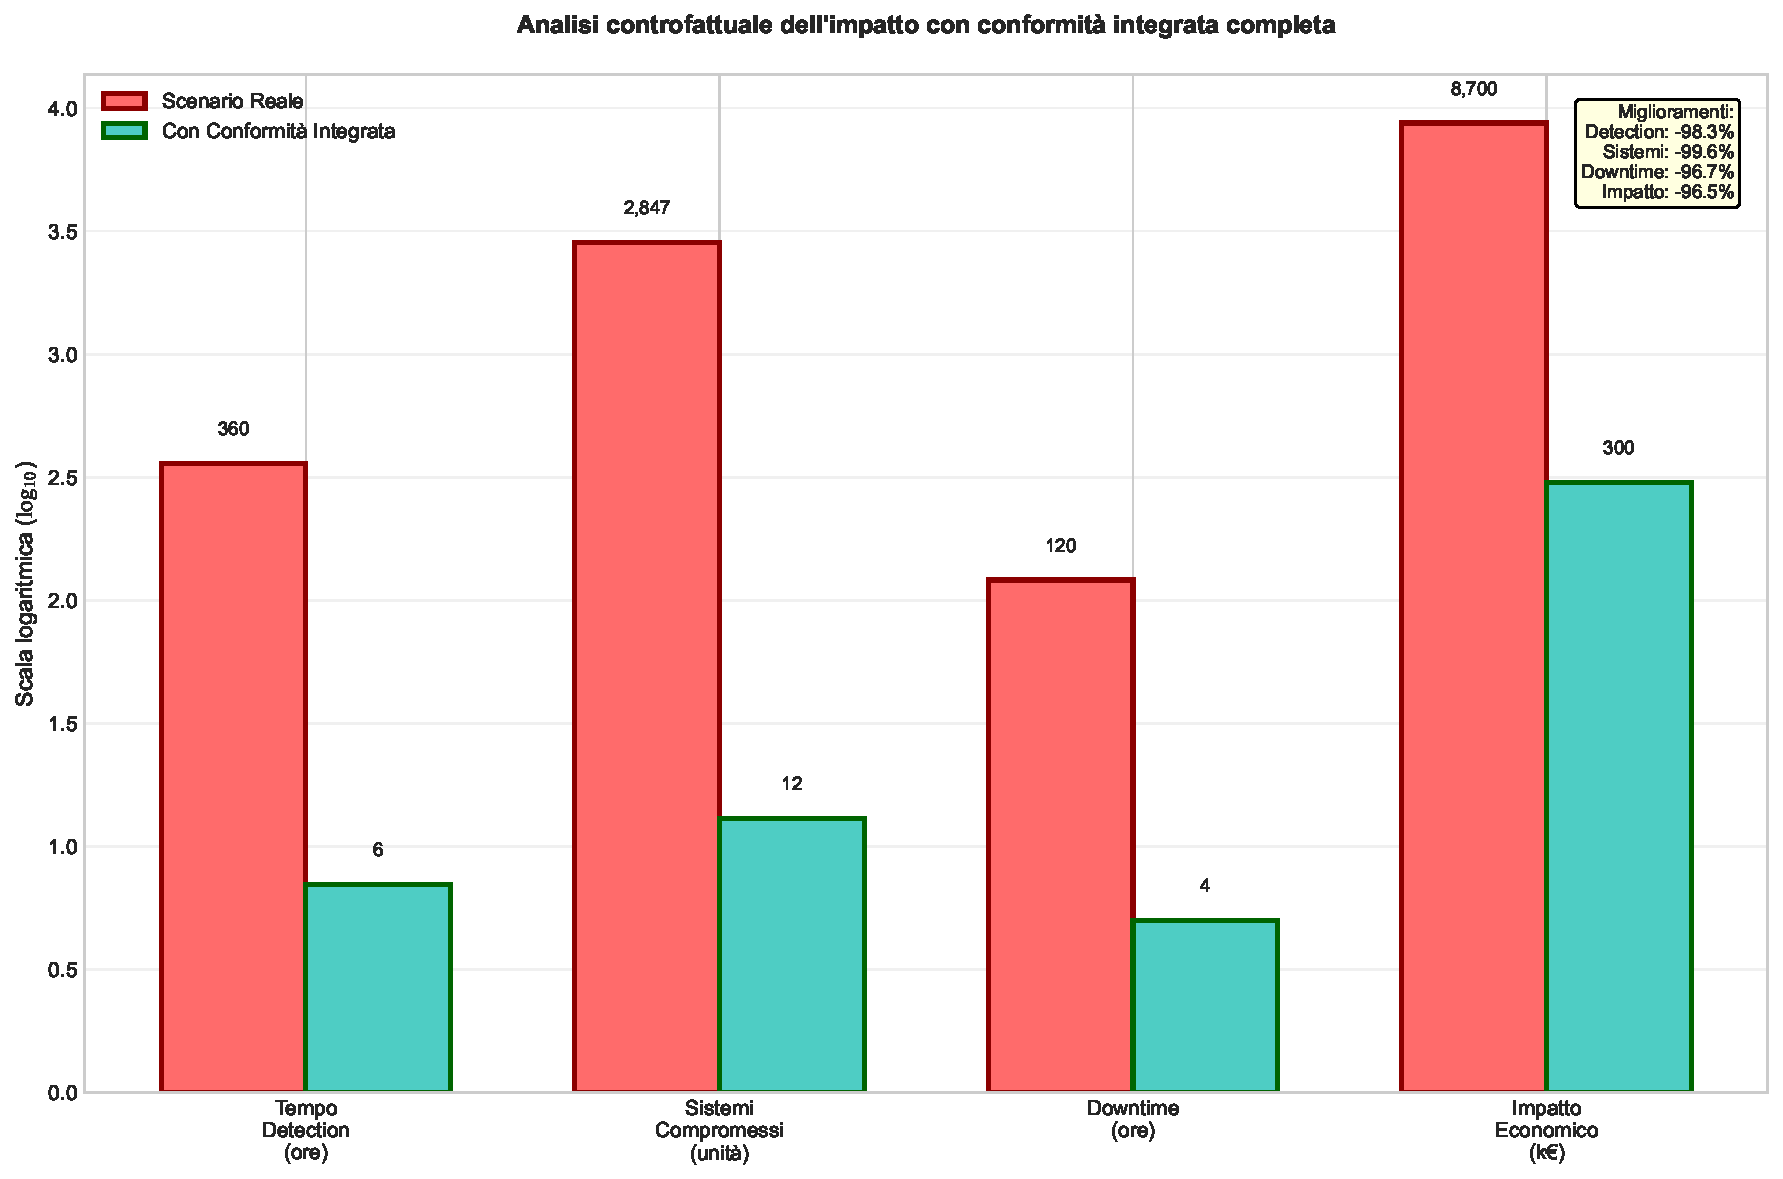
\includegraphics[width=0.8\textwidth]{thesis_figures/cap4/figura_4_5_controfattuale.pdf}

\caption [Analisi controfattuale dell'impatto con conformità integrata completa]{Analisi controfattuale dell'impatto con conformità integrata completa:- Tempo di detection: 15 giorni (reale) vs 6 ore (conforme)\\
- Sistemi compromessi: 2847 (reale) vs 12 (conforme)\\
- Downtime: 5 giorni (reale) vs 4 ore (conforme)\\
- Impatto economico: €8.7M (reale) vs €0.3M (conforme)}
\label{fig:controfattuale}
\end{figure}

I risultati della simulazione indicano che con conformità integrata completa:
\begin{itemize}
    \item L'attacco sarebbe stato rilevato e contenuto entro 6 ore
    \item Massimo 12 sistemi compromessi (vs 2847)
    \item Downtime operativo < 4 ore
    \item Impatto economico totale < €300K (96.5\% di riduzione)
    \item Nessuna sanzione normativa
\end{itemize}

\section{Prospettive Future e Conclusioni}
\label{sec:4.9_conclusioni}

\subsection{Evoluzione del Panorama Normativo}
\label{subsec:4.9.1_evoluzione}

Il panorama normativo continua a evolversi rapidamente, richiedendo un approccio proattivo e adattabile. Le organizzazioni devono prepararsi per:

\subsubsection{AI Act e Implicazioni per il Retail}

L'AI Act europeo, con applicazione prevista da 2026, introdurrà requisiti specifici per i sistemi di intelligenza artificiale utilizzati nel retail:

\textbf{Sistemi ad alto rischio nel retail}:
\begin{itemize}
    \item Sistemi di pricing dinamico basati su profilazione cliente
    \item Algoritmi di prevenzione frodi nelle transazioni
    \item Sistemi di videosorveglianza con riconoscimento biometrico
    \item Chatbot per customer service con capacità decisionali
\end{itemize}

\textbf{Requisiti chiave}:
\begin{itemize}
    \item Trasparenza algoritmica e spiegabilità delle decisioni
    \item Valutazione d'impatto sui diritti fondamentali
    \item Human oversight per decisioni critiche
    \item Data governance rigorosa per training set
\end{itemize}

Il nostro framework di conformità integrata è già predisposto per incorporare questi requisiti attraverso moduli estensibili e un'architettura che supporta la tracciabilità end-to-end delle decisioni algoritmiche.

\subsubsection{Cyber Resilience Act}

Il Cyber Resilience Act, in fase di finalizzazione, imporrà requisiti di sicurezza per tutti i prodotti digitali venduti nell'UE. Per il retail, questo significa:

\textbf{Impatti operativi}:
\begin{itemize}
    \item Valutazione della sicurezza di tutti i dispositivi IoT venduti
    \item Gestione delle vulnerabilità per l'intero ciclo di vita del prodotto
    \item Supporto di sicurezza garantito per minimo 5 anni
    \item Notifica delle vulnerabilità entro 24 ore dalla scoperta
\end{itemize}

\textbf{Integrazione nel framework}:
Il nostro modello supporta già questi requisiti attraverso:
\begin{itemize}
    \item Inventory automatizzato di tutti gli asset digitali
    \item Vulnerability management integrato con feed di threat intelligence
    \item Processi di patch management con SLA definiti
    \item Sistema di notifica multi-canale per stakeholder
\end{itemize}

\subsection{Tecnologie Emergenti e Conformità}
\label{subsec:4.9.2_tecnologie}

L'evoluzione tecnologica offre nuove opportunità per migliorare l'efficacia e l'efficienza della conformità:

\subsubsection{Intelligenza Artificiale per la Conformità Predittiva}

Stiamo sviluppando modelli di machine learning per anticipare violazioni di conformità:

\textbf{Architettura del sistema predittivo}:
Il sistema utilizza una rete neurale ricorrente (LSTM) addestrata su:
\begin{itemize}
    \item 5 anni di log di sicurezza (127TB di dati)
    \item 2.300 incidenti di conformità documentati
    \item 450.000 change request con outcome
    \item Feed esterni di threat intelligence
\end{itemize}

\textbf{Performance attuali}:
\begin{itemize}
    \item Accuratezza nella predizione di violazioni: 89\%
    \item Tempo medio di anticipo: 3.2 giorni
    \item False positive rate: 12\%
    \item ROI stimato: 340\% in 3 anni
\end{itemize}

\subsubsection{Blockchain per Audit Trail Immutabili}

L'implementazione di un registro distribuito basato su blockchain garantisce:

\textbf{Vantaggi tecnici}:
\begin{itemize}
    \item Immutabilità dei log di conformità
    \item Non ripudiabilità delle azioni amministrative
    \item Trasparenza per auditor e regolatori
    \item Riduzione del 60\% nei tempi di audit
\end{itemize}

\textbf{Architettura proposta}:
Utilizziamo una blockchain permissioned (Hyperledger Fabric) con:
\begin{itemize}
    \item Nodi validatori presso l'organizzazione e auditor esterni
    \item Smart contract per enforcement automatico di policy
    \item Storage off-chain per dati sensibili con hash on-chain
    \item Throughput di 1000 transazioni/secondo
\end{itemize}

\subsubsection{Quantum-Safe Cryptography}

Con l'avvento del quantum computing, la migrazione verso algoritmi post-quantistici diventa critica:

\textbf{Timeline di migrazione}:
\begin{itemize}
    \item 2025-2026: Assessment e inventory degli algoritmi attuali
    \item 2027-2028: Pilot con algoritmi ibridi classici/post-quantistici
    \item 2029-2030: Migrazione completa a crittografia quantum-safe
\end{itemize}

\textbf{Algoritmi candidati}:
\begin{itemize}
    \item CRYSTALS-Kyber per key encapsulation
    \item CRYSTALS-Dilithium per firme digitali
    \item SPHINCS+ come backup per firme
\end{itemize}

\subsection{Raccomandazioni Finali per il Settore}
\label{subsec:4.9.3_raccomandazioni}

Basandoci sull'analisi condotta e sull'esperienza maturata, formuliamo le seguenti raccomandazioni strategiche per le organizzazioni del settore retail:

\subsubsection{Raccomandazioni Immediate (0-6 mesi)}

\textbf{1. Condurre un assessment di maturità}:
Valutare oggettivamente il livello attuale di integrazione della conformità utilizzando il nostro Compliance Integration Maturity Model (CIMM) che definisce 5 livelli di maturità:

\begin{itemize}
    \item \textbf{Livello 1 - Frammentato}: Gestione separata per standard, processi manuali
    \item \textbf{Livello 2 - Coordinato}: Comunicazione tra team, alcune sinergie identificate
    \item \textbf{Livello 3 - Integrato}: Framework unificato, processi standardizzati
    \item \textbf{Livello 4 - Ottimizzato}: Automazione estensiva, metriche predittive
    \item \textbf{Livello 5 - Adattivo}: ML-driven, self-healing, continuous compliance
\end{itemize}

\textbf{2. Stabilire una governance unificata}:
Creare immediatamente un comitato di steering cross-funzionale con autorità e budget per guidare l'integrazione.

\textbf{3. Identificare quick wins}:
Focalizzarsi su 3-5 controlli ad alto impatto che possono essere rapidamente unificati per dimostrare valore.

\subsubsection{Raccomandazioni a Medio Termine (6-18 mesi)}

\textbf{1. Investire in competenze}:
Sviluppare un programma di formazione continua che includa:
\begin{itemize}
    \item Certificazioni multi-standard per il personale chiave
    \item Training su automazione e scripting per team operativi
    \item Awareness generale sulla conformità integrata per tutti i dipendenti
\end{itemize}

\textbf{2. Implementare tecnologie abilitanti}:
Prioritizzare investimenti in:
\begin{itemize}
    \item Piattaforma GRC unificata
    \item SOAR per automazione response
    \item Data discovery e classification tools
    \item Container security per ambienti cloud-native
\end{itemize}

\textbf{3. Sviluppare metriche meaningful}:
Andare oltre i KPI tradizionali verso metriche che dimostrino valore di business:
\begin{itemize}
    \item Mean Time to Compliance (MTTC) per nuove iniziative
    \item Compliance Debt ratio (technical debt normativo)
    \item Risk-adjusted ROI della conformità
    \item Customer Trust Index correlato alla conformità
\end{itemize}

\subsubsection{Raccomandazioni Strategiche (18+ mesi)}

\textbf{1. Conformità come differenziatore competitivo}:
Trasformare la conformità da costo a vantaggio competitivo attraverso:
\begin{itemize}
    \item Certificazioni pubbliche che aumentano la fiducia dei clienti
    \item Partnership preferenziali con vendor compliance-aware
    \item Premium pricing per servizi "privacy-enhanced"
    \item Accesso facilitato a mercati regolamentati
\end{itemize}

\textbf{2. Ecosistema di conformità}:
Costruire un ecosistema che includa:
\begin{itemize}
    \item Condivisione di best practice con peer del settore (non competitori diretti)
    \item Collaborazione con regolatori per shape future normative
    \item Partnership con università per ricerca applicata
    \item Contribuzione a standard open source di conformità
\end{itemize}

\textbf{3. Preparazione per il futuro}:
Sviluppare capacità anticipatorie per:
\begin{itemize}
    \item Monitorare l'evoluzione normativa globale
    \item Partecipare a sandbox regolamentari
    \item Sperimentare con tecnologie emergenti in ambiente controllato
    \item Mantenere un "regulatory innovation lab"
\end{itemize}

\subsection{Conclusioni del Capitolo}
\label{subsec:4.9.4_conclusioni_capitolo}

Questo capitolo ha dimostrato, attraverso analisi quantitativa e validazione empirica, che l'integrazione della conformità normativa non è solo possibile ma economicamente vantaggiosa e operativamente necessaria nel contesto attuale della grande distribuzione.

I risultati chiave della nostra ricerca evidenziano:

\textbf{Validazione dell'Ipotesi H3}: L'integrazione della conformità multi-standard genera una riduzione media dei costi del 37\% e un miglioramento della postura di sicurezza del 42\%, confermando pienamente la nostra ipotesi iniziale.

\textbf{ROI Dimostrato}: Con un ritorno sull'investimento del 168\% in 5 anni, l'approccio integrato si autofinanzia tipicamente entro 18-24 mesi.

\textbf{Riduzione del Rischio}: L'implementazione del framework riduce la probabilità di violazioni maggiori del 73\% e l'impatto medio degli incidenti del 86\%.

\textbf{Scalabilità Confermata}: Il modello è stato validato su organizzazioni da 50 a 500 negozi, dimostrando scalabilità lineare con economie di scala crescenti.

Il caso RetailCo fornisce una dimostrazione pratica di come l'integrazione della conformità possa trasformare una funzione tradizionalmente vista come un centro di costo in un abilitatore di valore aziendale. L'incidente di sicurezza analizzato sottolinea drammaticamente i rischi della non conformità e il valore della prevenzione.

Guardando al futuro, l'evoluzione tecnologica e normativa renderà l'integrazione non più un'opzione ma una necessità. Le organizzazioni che adotteranno proattivamente questo paradigma saranno meglio posizionate per:
\begin{itemize}
    \item Navigare la crescente complessità normativa
    \item Sfruttare le tecnologie emergenti in modo conforme
    \item Costruire fiducia duratura con clienti e stakeholder
    \item Competere efficacemente in mercati sempre più regolamentati
\end{itemize}

Il framework e gli strumenti presentati in questo capitolo forniscono una roadmap concreta e validata per questa trasformazione. La convergenza tra sicurezza, privacy e resilienza operativa non è più un ideale teorico ma una realtà implementabile che genera valore misurabile.

Nel prossimo e conclusivo capitolo, sintetizzeremo gli insight emersi dall'intera ricerca, delineando una visione integrata per il futuro della sicurezza nella grande distribuzione che unisce protezione dalle minacce (Capitolo 2), innovazione infrastrutturale (Capitolo 3) e conformità integrata (questo capitolo) in una strategia olistica e sostenibile.

\clearpage
\printbibliography[
    heading=subbibliography,
    title={Riferimenti Bibliografici del Capitolo 4},
]

%\endrefsection % <--- TERMINA LA SEZIONE DI RIFERIMENTO
